\documentclass[11pt, oneside]{article}   	

%%%%%%%%%%%%%%%%%%%%%%%%%%%%%%%%%%
% Packages
%%%%%%%%%%%%%%%%%%%%%%%%%%%%%%%%%%
\usepackage[colorlinks,citecolor=blue,urlcolor=blue,filecolor=blue,backref=page]{hyperref}

\usepackage[margin=1in]{geometry}           	
\geometry{a4paper}                   	

\usepackage{graphicx}	
\usepackage{float}
\usepackage{afterpage}
\usepackage{caption}
\usepackage{subcaption}
\usepackage{layouts}
\usepackage{tikz}
\usetikzlibrary{shapes, calc, shapes, arrows, positioning}


% \usepackage{setspace}
% \onehalfspacing
\linespread{1.5}

% \pdfpageattr {/Group << /S /Transparency /I true /CS /DeviceRGB>>}

\usepackage{amsthm}
\usepackage{amsmath}							
\usepackage{amssymb}
\usepackage{mathtools}

\usepackage[utf8]{inputenc}

\usepackage{natbib}

\usepackage{url}

\usepackage{commath}

\usepackage[super]{nth}

%%%%%%%%%%%%%%%%%%%%%%%%%%%%%%%%%%
% Macros
%%%%%%%%%%%%%%%%%%%%%%%%%%%%%%%%%%

\newcommand{\thetab}{{\boldsymbol{\theta}}}
\newcommand{\thetaHat}{{\hat{\thetab}}}
\newcommand{\alphab}{{\boldsymbol{\alpha}}}
\newcommand{\betab}{{\boldsymbol{\beta}}}
\newcommand{\mub}{\boldsymbol{\mu}}
\newcommand{\Sigmab}{\boldsymbol{\Sigma}}
\newcommand{\xib}{{\boldsymbol{\xi}}}
\newcommand{\xitildeb}{{\boldsymbol{\tilde{\xi}}}}
\newcommand{\pnorm}{p}
\newcommand{\pnn}{\phi}
\newcommand{\pnnj}{f}
\newcommand{\pdata}{p_{ \mathbf x}}
\newcommand{\pnoise}{p_{ \mathbf y}}
\newcommand{\pcondnoise}{p_{\y|\x}}
\newcommand{\palpha}{p_\alphab}
\newcommand{\pbeta}{p_\betab}
\newcommand{\q}[1]{q(\z \given{#1})}
\newcommand{\gradtheta}{\nabla_{\thetab}}

\newcommand{\Ib}{\boldsymbol{I}}
\renewcommand{\u}{{\mathbf u}}
\newcommand{\x}{{\mathbf x}}
\newcommand{\y}{{\mathbf y}}
\newcommand{\z}{{\mathbf z}}
\newcommand{\w}{{\mathbf w}}
\newcommand{\ytilde}{\mathbf{\tilde{y}}}
\newcommand{\X}{{\mathbf X}}
\newcommand{\N}{\mathcal{N}}
\newcommand{\I}{{\mathbb I}}
\newcommand{\psib}{\boldsymbol{\psi}}


\renewcommand{\P}{\mathbb{P}}
\newcommand{\E}{\mathbb{E}}
\newcommand{\Ex}{\E_{\x}}
\newcommand{\Ey}{\E_{\y}}
\newcommand{\Edata}{\E_{\x \sim p^*}}
\newcommand{\Evar}[1]{\E_{\z \sim \q{#1}}}
\newcommand{\Ealpha}{\mathbb{E}_{\alphab}}
\newcommand{\Ebeta}{\mathbb{E}_{\betab}}
\newcommand{\J}{\mathcal{J}}

% for conditional probabilities / expectations
\newcommand\given[1][]{\:#1\vert\:}

% KL-divergence double bar with: \infdiv{KL}{p}{q}
\DeclarePairedDelimiterX{\infdivx}[2]{(}{)}{%
#1\;\delimsize\|\;#2%
}
\newcommand{\infdiv}[1]{D_{#1}\infdivx}
\DeclarePairedDelimiter{\norm}{\lVert}{\rVert}

\newtheorem{theorem}{Theorem}
\newtheorem{corollary}{Corollary}[theorem]
\newtheorem{lemma}[theorem]{Lemma}

\theoremstyle{definition}
\newtheorem{definition}{Definition}[section]

\newcommand{\argmax}[1]{\underset{#1}{\operatorname{arg}\,\operatorname{max}}\;}

\tikzstyle{neuron}=[draw,circle,minimum size=20pt,inner sep=0pt, fill=white]
\tikzstyle{stateTransition}=[thick]
\tikzstyle{learned}=[text=red]




%%%%%%%%%%%%%%%%%%%%%%%%%%%%%%%%%%
% Latex settings
%%%%%%%%%%%%%%%%%%%%%%%%%%%%%%%%%%

\graphicspath{{./figs/}}


%%%%%%%%%%%%%%%%%%%%%%%%%%%%%%%%%%
% Text
%%%%%%%%%%%%%%%%%%%%%%%%%%%%%%%%%%

\title{Variational Noise-contrastive Estimation}
\author{Ben Rhodes}
\date{\today}						

\begin{document}
\maketitle


%%%%%%%%%%%%%%%%%%%%%%%%%%%%%%%%%%%%%%%%%%%%%%%%%%%%%%%%%%%%%%%%%%%%%%%%%%%%%%%%%%%%%%%%%%%%%%%%%%%%%%%%%%%%%%%%%%%%%
%                                        ABSTRACT
%%%%%%%%%%%%%%%%%%%%%%%%%%%%%%%%%%%%%%%%%%%%%%%%%%%%%%%%%%%%%%%%%%%%%%%%%%%%%%%%%%%%%%%%%%%%%%%%%%%%%%%%%%%%%%%%%%%%%

\section{Abstract}
This thesis presents a method for estimating the parameters of unnormalised probability densities with unobserved (or `latent’) variables. The method is an extension of noise-contrastive estimation, which applies only to unnormalised, fully observed models.


%%%%%%%%%%%%%%%%%%%%%%%%%%%%%%%%%%%%%%%%%%%%%%%%%%%%%%%%%%%%%%%%%%%%%%%%%%%%%%%%%%%%%%%%%%%%%%%%%%%%%%%%%%%%%%%%%%%%%
%                                        INTRODUCTION
%%%%%%%%%%%%%%%%%%%%%%%%%%%%%%%%%%%%%%%%%%%%%%%%%%%%%%%%%%%%%%%%%%%%%%%%%%%%%%%%%%%%%%%%%%%%%%%%%%%%%%%%%%%%%%%%%%%%%
% \printinunitsof{in}\prntlen{\linewidth}
\section{Introduction}
\textbf{An unnormalised model}, $\pnn(\u;\thetab)$, is a parametrised family of non-negative functions that you can think of as scaled probability density \footnote{unless stated otherwise, assume that all results apply equally to probability mass functions defined over discrete random variables, replacing integrals with sums as necessary.} functions that do not integrate to 1 for all values of $\thetab$. That is:
 \begin{align}
   \int_{\u }\pnn(\u;\thetab) \dif \u &= Z(\thetab) \neq 1 & \pnn(\u;\thetab) \geq 0
\label{eq:Zdef}
  \end{align}
where $Z(\thetab$) is called the \emph{partition function}. The partition function is important because it allows us to normalise $\pnn(\u;\thetab)$, obtaining a model $\pnorm(\u; \thetab)$ that, regardless of the value of $\thetab$, integrates to 1.
\begin{align}
  \pnorm(\u;\thetab)&=\frac{\pnn(\u;\thetab)}{Z(\thetab)}, & \int_{\u }\pnorm(\u;\thetab) \dif\u & = 1.
  \label{unnormalised density}
\end{align}
Unfortunately, the partition function is rarely computable analytically, and the cost of approximating it generally scales exponentially with the dimension of $\u$. The intractability of the partition function becomes problematic when we want to estimate good values of $\thetab$ given some data $\{\x_1, ..., \x_n\}$, where `good' --- in practical terms --- means that  $\pnorm(\x_i; \thetab)$ is large for all $i$ (whilst still satisfying the constraint of integrating to 1). It is problematic because the standard approach of maximum likelihood estimation requires us to maximise an objective that depends on the partition function; namely, the log-likelihood:
\begin{align}
\ell_n(\thetab) &= \sum_{i=0}^{n}  \log \pnorm(\x_i;\thetab) = \sum_{i=0}^{n}  \log \pnn(\x_i;\thetab) - n \log ( Z(\thetab) ),
\label{eq:log-likelihood}
\end{align}
To handle this intractability, multiple methods for estimating the parameters $\thetab$ without directly computing the partition function, such as pseudolikelihood \citep{besag1975statistical}, score matching \citep{hyvarinen2005estimation}, ratio matching \citep{hyvarinen2007some}, contrastive divergence \citep{hinton2006training}, persistent contrastive divergence \citep{younes1998stochastic, tieleman2009using} and noise-contrastive estimation (NCE) \citep{gutmann2012noise}. The final three methods --- contrastive divergence, its persistent variant, and NCE --- are perhaps the most versatile, being simple to implement and applicable to a large class of models. In some respects, NCE is preferable to contrastive divergence since it has a well-defined objective function (a point we shall return to later) and, under some quite general assumptions, is guaranteed to converge to the true value of $\thetab$. However, NCE cannot currently be applied to models with hidden, or \emph{latent}, variables, whereas contrastive divergence can. It is this deficiency of NCE that this thesis aims to remedy.

\textbf{A latent variable model} is a family of probability densities $\pnorm(\u; \thetab)$ for which we do not have a direct expression; instead we only have a joint $\pnorm(\u, \z; \thetab)$ density, where $\z$ are hidden variables, not present in our data set. We thus obtain $\pnorm(\u; \thetab)$ only after marginalisation:
\begin{align}
  \pnorm(\u; \thetab) = \int \pnorm(\u, \z;\thetab) \dif \z \ .
  \label{eq:marginal}
\end{align}

Learning the parameters $\thetab$ is problematic here for essentially the same reason as in unnormalised models: the presence of an intractable integral. In section \ref{sec:VNCE} we discuss a general strategy for overcoming this intractability using variational inference.

To see why latent variable models are important, it helps to consider two conceptually distinct (but mathematically equivalent) types of latent variables. The first type represent `missing data’; perhaps certain pixels in an image were corrupted, generating NaNs. The second type represent compressions of the visible data, which often (but not always) capture low-dimensional causes of the visible data. Such compressions are at the core of unsupervised learning, since the ability to build parsimonious models of the hidden causes of your observations appears to be a fundamental aspect of intelligence. Thus, it is primarily the second view of latent variables that motivates the widespread use of such models. 

Let us now consider the combined case of an unnormalised, latent variable model. To write down an expression for $\pnorm(\u; \thetab)$, we combine equations \ref{unnormalised density} and \ref{eq:marginal} to get:
\begin{align}
    \pnorm(\u; \thetab) = \frac{\int \pnn(\u, \z;\thetab) \dif \z}{Z(\thetab)} \ ,
\end{align}
where $Z(\thetab)$ is as we defined it in equation \ref{eq:Zdef}. This expression contains two troublesome integrals, and it is this double intractability that is the fundamental technical barrier we must overcome to perform parameter estimation.

\newpage
\section{Background}

%%%%%%%%%%%%%%%%%%%%%%%%%%%%%%%%%%%%%%%%%%%%%%%%%%%%%%%%%%%%%%%%%%%%%%%%%%%%%%%%%%%%%%%%%%%%%%%%%%%%%%%%%%%%%%%%%%%%%
%                                            MLE
%%%%%%%%%%%%%%%%%%%%%%%%%%%%%%%%%%%%%%%%%%%%%%%%%%%%%%%%%%%%%%%%%%%%%%%%%%%%%%%%%%%%%%%%%%%%%%%%%%%%%%%%%%%%%%%%%%%%%

\subsection{Maximum Likelihood}
\label{sec:mle}
As stated in the introduction, maximum likelihood learning consists of maximising the log-likelihood given in equation \ref{eq:log-likelihood}, which is a summation over $n$ data points. However, for much of the theory presented in this thesis, it will be convenient to remove the dependency on a finite set of data, and just refer to the underlying distributions that generate the data. To do this, note that the average log-likelihood is the sample version of:
\begin{align}
\label{eq:expectation log-like}
\ell(\thetab) &= \Edata \left[ \log \pnorm(\x;\thetab) \right].
\end{align}
For many applications, this expression for the average log-likelihood can be used directly for learning the parameters $\thetab$. However, we are interested in latent variable, unnormalised models and so a more convenient expression is:
\begin{align}
\ell(\thetab) &= \Edata \left[\log \pnn(\x;\thetab) \right] - \log Z(\thetab) \\
              &= \Edata \left[ \log \int\pnn(\x, \z;\thetab) \dif \z \right] - \log \int\pnn(\x, \z;\thetab) \dif \x \dif \z \ ,
\end{align}
where $p^*$ is the data generating distribution. One can show that the gradient of $\ell(\thetab)$ is given by:
\begin{align}
    \label{eq:unnormalised latent var mle gradient}
    \gradtheta \ell(\thetab) = \Edata \E_{\z \sim p(\z \given \x)} \left[ \gradtheta \log \pnn(\x, \z;\thetab) \right] - \E_{\x, \z \sim p(\x, \z)} \left[\gradtheta \log \left(\pnn(\x, \z;\thetab) \right) \right] \ ,
\end{align}
Intuitively, the first gradient `pushes up' on $\pnn$ wherever the \emph{data} is likely, whilst the second term `pushes down' on  $\pnn$ wherever the \emph{model} is likely. The net effect is to reallocate probability mass from regions where the data is unlikely to regions where it is likely. It is critical that we \emph{reallocate} mass, and not simply increase the total amount, since the model must integrate to one. At equilibrium, these two forces directly cancel, and the model equals the data generating distribution.


In general, the expectations in equation \ref{eq:unnormalised latent var mle gradient} will not be computable analytically. Then the question becomes, can we efficiently sample from the model's posterior over latents $p(\z \given \x)$ and the from the joint $p(\x, \z)$? Sampling must be efficient since we need to re-sample after \emph{every} gradient update. For many models of interest, such as the Restricted Boltzmann Machine discussed in \ref{sec:rbm}, sampling from $p(\z \given \x)$ is straightforward, whilst sampling from the joint $p(\x, \z)$ is problematic. The reason is that many unnormalised, latent variable models are defined via undirected graphs, which do not permit ancestral sampling and generally require us to use a Monte-Carlo Markov Chain (MCMC) method that can be very slow to converge.

\subsection{Contrastive Divergence}
\label{sec:cd}
Contrastive divergence \citep{hinton2006training} bypasses the slow MCMC sampling needed for maximum likelihood in equation \ref{eq:unnormalised latent var mle gradient} by initialising the Markov chain at a data point and only running it for k-steps (rather than waiting for it to converge), where k is a tuning hyperparameter. Thus, the gradient updates are given by:
\begin{align}
    \label{eq:cd grad update}
    \nabla_{\thetab} \ell(\thetab) &= \Edata \E_{\z \sim p(\z \given \x)} \left[ \nabla_{\thetab} \log \pnn(\x, \z;\thetab) \right] - \E_{\x, \z \sim p_k(\x, \z)} \left[\nabla_{\thetab} \log \left(\pnn(\x, \z;\thetab) \right) \right] \ , 
\end{align}
where $p_k$ is the distribution obtained after running the Markov chain for k steps, starting at a datapoint. \citet{bengio2009justifying} showed that the difference between the MLE gradient update and the contrastive divergence update, given by 
\begin{equation}
    \label{eq:cd bias}
    \E_{\x \sim p_k(\x)} \left[ \gradtheta \log p_k(\x) \right] \ ,
\end{equation}
tends to zero as k tends to infinity and in the specific case of the RBM, provided a bound on this term. Non model-specific bounds seem hard to derive, and little is known in general about the convergence properties of contrastive divergence \citep{carreira2005contrastive}. One interesting result we do have is that the contrastive divergence update is \emph{not} the update of any objective function \citep{sutskever2010convergence}, which prevents us applying non-linear optimisation methods. Despite the weak theory supporting contrastive divergence, it has proven empirically to be an efficient learning technique in many situations.

A related learning method to contrastive divergence is  \emph{persistent} contrastive divergence \citep{younes1998stochastic, tieleman2009using}. Instead of initialising the Markov chains at a datapoint after every gradient update, we `persist' the state of the chain and reuse it across gradient steps. 

%%%%%%%%%%%%%%%%%%%%%%%%%%%%%%%%%%%%%%%%%%%%%%%%%%%%%%%%%%%%%%%%%%%%%%%%%%%%%%%%%%%%%%%%%%%%%%%%%%%%%%%%%%%%%%%%%%%%%
%                                       STANDARD VARIATIONAL INFERENCE
%%%%%%%%%%%%%%%%%%%%%%%%%%%%%%%%%%%%%%%%%%%%%%%%%%%%%%%%%%%%%%%%%%%%%%%%%%%%%%%%%%%%%%%%%%%%%%%%%%%%%%%%%%%%%%%%%%%%%

\subsection{Variational inference and EM}
Variational inference \citep{jordan1999introduction} is a method for turning probabilistic inference of latent variables into an optimisation problem. This optimisation problem then leads to efficient, scalable algorithms for learning the parameters of latent variable models. To see how this works, we return to the average log-likelihood objective function presented in section \ref{sec:mle}, which for a latent variable model is given by:
\begin{align}
    \ell(\thetab) &= \Ex  \log \left( \int \pnorm(\x, \z;\thetab) \dif \z  \right)  \\
                  &= \Ex \log \left( \Evar{\x} \left( \frac{\pnorm(\x, \z;\thetab)}{\q{\x}} \right)  \right)
\end{align}
where, in the second line, we applied a simple identity known as importance sampling, where the `auxiliary' density $q$ can be any valid density that is non-zero whenever $\pnorm$ is non-zero. We then apply Jensen's inequality, using the fact that the $\log$ function is concave, giving:
\begin{align}
    \ell(\thetab) &\geq \Ex \Evar{\x} \left( \log \left( \frac{\pnorm(\x, \z;\thetab)}{\q{\x}} \right) \right) \ .
    \label{eq:elbo}
\end{align}
It is straightforward to show that this inequality is tight when $\q{\x} = \pnorm(\z \given \x; \thetab)$. This inequality directly leads to an iterative algorithm, known as Expectation Maximisation (EM) for estimating the parameters $\thetab$. Whilst the idea of EM is quite old, originally by \citet{dempster1977maximum}, the view presented here is similar to that given by \citet{neal1998view}. The algorithm simply involves alternating between optimising the right-hand side of equation \ref{eq:elbo} with respect to $\thetab$ (which we can do since we have an expression for $\pnorm(\x, \z;\thetab)$) and then, with our new $\thetab$, setting: $\q{\x} = \pnorm(\z \given \x; \thetab)$. One can prove that this iterative algorithm always increases the log-likelihood.

EM, as stated above, assumes we have an expression for $\pnorm(\z \given \x; \thetab)$. That is, we assume \emph{inference} of the latent variables is tractable. What if this is not the case? Well, we still want $q$ to approximate the posterior over latent variables, and so we could parametrise it with parameters $\alphab$. If this parametric family is sufficiently broad, we might hope that one of its members is close to the true posterior, and that we can find such a member by optimising $\alphab$. Thus, instead of resetting: $\q{\x} = \pnorm(\z \given \x; \thetab)$, we optimise the right-hand side of \ref{eq:elbo} with respect to the \emph{variational parameters} $\alphab$.

How to perform this optimisation with respect to $\alphab$ is a matter of ongoing research. It is non-trivial because the right-hand side of $\ref{eq:elbo}$ involves an expectation with respect to $q(\z \given\x; \alphab)$, so standard gradient-based methods are hard to straightforwardly apply. There are methods to cope with this obstacle, such as the reparameterisation trick \citep{kingma2015variational}, which we discuss in later chapters. 
%%%%%%%%%%%%%%%%%%%%%%%%%%%%%%%%%%%%%%%%%%%%%%%%%%%%%%%%%%%%%%%%%%%%%%%%%%%%%%%%%%%%%%%%%%%%%%%%%%%%%%%%%%%%%%%%%%%%%
%                                           INTRO TO NCE
%%%%%%%%%%%%%%%%%%%%%%%%%%%%%%%%%%%%%%%%%%%%%%%%%%%%%%%%%%%%%%%%%%%%%%%%%%%%%%%%%%%%%%%%%%%%%%%%%%%%%%%%%%%%%%%%%%%%%
\subsection{Noise-contrastive estimation}
\label{sec:nce}
NCE converts an unsupervised density estimation problem into a supervised classification problem, by training a (non-linear) logistic classifier to distinguish between the true data and samples from some reference distribution, which we refer to as noise samples.

Concretely, we first generate $m$ samples $\{\textbf{y}_1, \ldots \textbf{y}_m\}$ from a noise distribution $\pnoise(\textbf{y})$ and mix these samples with our data $(\textbf{x}_1, …., \textbf{x}_n)$. Our goal is now to classify whether a random sample $\u$ from this mixture came from the data-generating distribution $p$ or the noise $\pnoise$. We do so by calculating posterior probabilities, using our unnormalised model $\phi(\u; \thetab)$ as a surrogate for the true probability of the data $p(\u)$. If $\nu = \frac{m}{n}$, then:
\begin{align}
    \color{red}{\P( \u \sim \pdata; \thetab)} &= \color{red}{\frac{\pnn(\textbf{u}; \thetab)}{\pnn(\textbf{u}; \thetab) + \nu \pnoise(\textbf{u})}} \\
    \color{blue}{\P( \u \sim \pnoise; \thetab)} &= \color{blue}{\frac{\nu \pnoise(\textbf{u})}{\pnn(\textbf{u}; \thetab) + \nu \pnoise(\textbf{u})}.}
\end{align}
Note that $\P( \u \sim \pnoise; \thetab ) = 1 - \P( \u \sim \pdata; \thetab )$, which makes sense because this is a two-class classification problem, and so we have a Bernoulli distribution over the class label. Using the average log-likelihood for a Bernoulli, we derive the following objective function:
\begin{align}
  J_n(\thetab)&= 
  \frac{1}{n} \left\{ \color{red}{\sum_{i=1}^{n} \log  \P( \x_i \sim \pdata; \thetab)} 
    + \color{blue}{\sum_{i=1}^{m} \log\left[\P( \y_i \sim \pnoise; \thetab )\right]} \right\} \\
  & = \color{red}{\frac{1}{n} \sum_{i=1}^{n} \log \left(\frac{\pnn(\x_i; \thetab)}{\pnn(\x_i; \thetab) + \nu \pnoise(\x_i)}\right)}
    + \color{blue}{\frac{1}{n}\sum_{i=1}^{m} \log \left(\frac{\nu \pnoise(\y_i)}{\pnn(\y_i; \thetab) + \nu \pnoise(\y_i)}\right),} 
  \label{eq:Jn}
\end{align}
which is the sample version of $J(\thetab)$:
\begin{equation}
  J(\thetab) = 
   \color{red}{\Ex  \log \left(\frac{\pnn(\x; \thetab)}{\pnn(\x; \thetab) + \nu \pnoise(\x)}\right)}
  + \color{blue}{\nu \Ey \log \left( \frac{\nu \pnoise(\y)}{\pnn(\y; \thetab) + \nu \pnoise(\y)}\right).}
  \label{eq:J}
\end{equation}

If we denote the true data generating distribution by $\pnorm(\u; \theta*)$, and assume that this distribution is contained within our unnormalised family $\phi(\u;\thetab)$, then, under some rather general technical conditions described by \citet{gutmann2012noise}, optimising $J(\thetab)$ guarantees that $\thetab$ converges (in probability) to $\theta^*$ in the limit of infinite data.

Why should the \emph{normalised} data generating distribution live in an \emph{unnormalised} family? This assumption may seem odd at first, but note that it is simple to give the model family $\pnn(\u; \thetab)$ an extra degree of freedom by multiplying it with a scaling parameter $c$. This new parameter is estimated in conjunction with $\thetab$, so that we automatically obtain a normalised solution.\footnote{note, this is \emph{not} the same as normalising the model i.e.\ computing the partition function, which provides the normalisation constant for \emph{every} value of $\thetab$}

It turns out that for a large number of noise samples, $\nu$, the choice of noise distribution $q$ is not important. However, increasing $\nu$ uses more computational resource, so we still need to select an appropriate distribution. It remains an area of active research to select a noise distribution $\pnoise$ based on theoretically justified properties, with the main constraints currently being that it should be cheap to sample from, non-zero wherever $\pnn$ is non-zero, and similar to the underlying the data generating distribution.

In the case of latent variable models, the extended version of NCE that we present in this thesis is able to partially automate the construction of a suitable noise distribution, which is a significant advance over hand-crafted choices.


%%%%%%%%%%%%%%%%%%%%%%%%%%%%%%%%%%%%%%%%%%%%%%%%%%%%%%%%%%%%%%%%%%%%%%%%%%%%%%%%%%%%%%%%%%%%%%%%%%%%%%%%%%%%%%%%%%%%%
%                                        INTRO TO VNCE
%%%%%%%%%%%%%%%%%%%%%%%%%%%%%%%%%%%%%%%%%%%%%%%%%%%%%%%%%%%%%%%%%%%%%%%%%%%%%%%%%%%%%%%%%%%%%%%%%%%%%%%%%%%%%%%%%%%%%
\newpage
\section{Variational noise-contrastive estimation}
\label{sec:VNCE}
Guttmann [2018, unpublished] derived a \emph{variational} lower bound to the NCE objective function, which is the mathematical keystone to this thesis. Inspired by the derivation of the variational lower bound for the log-likelihood (\ref{eq:elbo}), we apply a similar strategy to bounding the NCE objective function in equation \ref{eq:J}. There are two fundamental steps: 
\begin{itemize}
    \item Use importance sampling to re-express the intractable integral over $\z$ as an expectation; call this E.
    \item Apply Jensen’s inequality to a concave function g(E).
\end{itemize}
One complication in applying such a strategy is that the intractable integral $\int \pnn(\u, \z;\thetab) \dif \z$ appears both inside the expectation with respect to the data:
\begin{align}
    \color{red}{\Ex  \log \left(\frac{\int \pnn(\x, \z;\thetab) \dif \z}{\int \pnn(\x, \z;\thetab) \dif \z + \nu \pnoise(\x)}\right)}
    \label{eq:J term1}
\end{align}
and it also appears in the second term, which is an expectation with respect to the noise distribution:
\begin{align}
    \color{blue}{\nu \Ey \log \left( \frac{\nu \pnoise(\y)}{\int \pnn(\y, \z;\thetab) \dif \z + \nu \pnoise(\y)}\right).}
    \label{eq:J term2}
\end{align}
Let us focus only on the first term (\ref{eq:J term1}). Introducing the notation:
\begin{equation}
  r(\x;\thetab) = \frac{\int \pnn(\x, \z;\thetab) \dif \z}{\pnoise(\x)} = \Evar{\x} \left( \frac{\pnn(\x, \z;\thetab)}{\q{\x}\pnoise(\x)} \right)
  \label{eq:r-def}
\end{equation}
and
\begin{equation}
  g(r) = -\log \left(1+\nu \frac{1}{r} \right),
\end{equation}
we see that:
\begin{align}
    \color{red}{\log \left(\frac{\int \pnn(\x, \z;\thetab) \dif \z}{\int \pnn(\x, \z;\thetab) \dif \z + \nu \pnoise(\x)}\right)} 
    &= \color{red}{- \log \left( 1 + \nu \frac{\pnoise(\x)}{\int \pnn(\x, \z;\thetab) \dif \z}\right)} \\
    &=   \color{red}{g(r(\x; \thetab)).}
\end{align}
It quickly follows from lemma \ref{lemma: f convex} (see appendix) that $g$ is a concave function of $r$. Since $r$ is really just an expectation, as is clear from \ref{eq:r-def}, we can apply Jensen's inequality:
\begin{align}
 \color{red}{g(r(\x; \thetab))}  
    &\geq  \color{red}{\Evar{\x} g \left( \frac{\pnn(\x, \z;\thetab)}{\q{\x}\pnoise(\x)} \right)} \\
    &\geq  \color{red}{-\Evar{\x} \log \left(1+\nu \frac{\q{\x}\pnoise(\x)}{\pnn(\x,\z; \thetab)}\right)}  \\
    &\geq  \color{red}{\Evar{\x} \log \left( \frac{\pnn(\x,\z; \thetab)}{\pnn(\x,\z; \thetab) + \nu\q{\x}\pnoise(\x)} \right),} 
\end{align}
where, to get the last line, we simply substitute in the definition of $g$.

It does not appear possible to apply the same combination of importance sampling and Jensen's inequality to the second term of the NCE objective (\ref{eq:J term2}). However, we don’t necessarily need to. The intractable integral in the second term can be approximated just with importance sampling, \emph{re-using} the variational distribution $q$ that we got from the first term. Thus, we obtain a variational lower bound to the NCE objective function given by:
\begin{equation}
  \J_1(\thetab, q) 
  = \color{red}{\Ex \Evar{\x} \log \left( \frac{\pnn(\x,\z; \thetab)}{\pnn(\x,\z; \thetab) + \nu\q{\x}\pnoise(\x)} \right)}
   \color{blue}{ + \nu \Ey \log \left( \frac{\nu\pnoise(\y)}{\nu\pnoise(\y) + \E_{\z \sim q(\z \given \y)} \left[\frac{\pnn(\y,\z; \thetab)}{q(\z \given \y)} \right]}  \right).}
  \label{eq:vnce objective}
\end{equation}
We have that $J(\thetab) \ge \J_1(\thetab, q)$ for all $q$, and so we can apply variational EM, maximising $J(\thetab)$ by iterating between maximising $\J_1(\thetab,q)$ with respect to $\thetab$, and the tightening of the bound by maximising $\J_1(\thetab,q)$ with respect to the variational distribution $q$.


\subsection{Necessary ingredients to apply VNCE}
\label{sec:optimisation of var objective}
Having established the objective function \ref{eq:vnce objective} for VNCE, it is helpful to explicitly lay out the ingredients required for optimising it. We require:
\begin{itemize}
    \item A noise distribution over the visible variables $\pnoise$. This density should, ideally, be cheap to evaluate and sample from, and similar to the data distribution.
    \item A variational distribution over latent variables $q$. This will typically have its own parameters $\alphab$, apart from the case where we set $q$ to equal the model's posterior over latents. This is only possible for models with tractable posteriors. 
    \item If the variational distribution $q$ has parameters $\alphab$, then we need compute $\nabla_{\alphab} J_1(\alphab)$. This is difficult in general, but depending on the parameterisation of $q$, it may be possible to do analytically, perhaps using the reparameterisation trick \citep{kingma2015variational}.
    \item The gradient $\nabla_{\thetab} J_1(\thetab)$. A derivation of this gradient is given in the appendix, section \ref{sec:appendix grad of J1}. The key term required to compute it is the gradient of the logarithm of the unnormalised model: $\nabla_{\thetab}(\log \phi(\u; \thetab))$.
\end{itemize}


%%%%%%%%%%%%%%%%%%%%%%%%%%%%%%%%%%%%%%%%%%%%%%%%%%%%%%%%%%%%%%%%%%%%%%%%%%%%%%%%%%%%%%%%%%%%%%%%%%%%%%%%%%%%%%%%%%%%%
%                                        RESEARCH OBJECTIVES
%%%%%%%%%%%%%%%%%%%%%%%%%%%%%%%%%%%%%%%%%%%%%%%%%%%%%%%%%%%%%%%%%%%%%%%%%%%%%%%%%%%%%%%%%%%%%%%%%%%%%%%%%%%%%%%%%%%%%
\newpage
\section{Research Objectives}
\label{sec:research objectives}
In the previous section, we established a method of parameter estimation for unnormalised, latent variable models involving the maximisation of a variational lower bound to the NCE objective function, as given in equation \ref{eq:vnce objective}. We will refer to this method as VNCE. The over-arching goal in the remainder of the thesis is to appraise the usefulness of VNCE across different models, data sets, and evaluation metrics. In addition, we aim to contribute a better theoretical understanding of the new estimation method, which may involve studying its asymptotic properties or its mathematical similarities with other methods such as contrastive divergence.

\subsection{Models and data sets}
The first steps, which are ongoing, involve applying the estimator to models of different levels of complexity with synthetic data. To this end, we have investigated a simple unnormalised mixture of two gaussians, discussed in section \ref{sec:mog}, and a more sophisticated model: the Restricted Boltzmann Machine (RBM), discussed in section \ref{sec:rbm}. The RBM has received a significant amount of attention over the last 15 years in the machine learning community, and there is thus a wealth of published material on estimating its parameters. A natural first step is to therefore build on this work.

After experimenting on synthetic data, we will then apply an RBM to real data. Some of the most thorough empirical work to date on different methods for learning RBMs \citep{marlin2010inductive} considered a range of data sets such as MNIST\footnote{http://yann.lecun.com/exdb/mnist}, the small 20-Newsgroups data set\footnote{http://www.cs.toronto.edu/roweis/data.html} and an image dataset from CalTech101\footnote{http://www.vision.caltech.edu/Image\_Datasets}. It makes sense to evaluate the new estimation method on the same data sets, to enable straightforward comparisons of my results with the published literature. That said, one important finding by \citet{marlin2010inductive} was that comparisons of estimation methods does vary significantly depending on the data set, and so I will consider experimenting with an even greater variety of data later in the thesis, assuming the preliminary results warrant further investigation.

\subsection{Evaluation metrics}
There are many possible metrics to consider. Of particular interest are the quality of the probabilistic model (\emph{does it assign high probability to the test data?}), the asymptotic properties of the estimator (\emph{does it use data efficiently?}) and the computational cost of the estimator (\emph{does it converge quickly?}).

With regards to the quality of the probabilistic model, we want to know: is it close to the true data generating distribution? One way of measuring closeness between distributions is the KL divergence. We can estimate the KL divergence between the true distribution and our model by evaluating the model's log-likelihood on the test data. For relatively simple, low-dimensional models, where we can analytically solve for the partition function and marginal distribution over observed variables, we can indeed use the log-likelihood as an evaluation metric. For more complex models, we must resort to approximations of the log-likelihood.

With regards to asymptotic properties, it helps to consider the case of ordinary NCE. There it was proven that the estimator converges (in distribution) to a normal distribution centred on the true parameter value, in the limit of infinite data. It is natural to wonder if a similar result might hold in our case. That is, do we have:
\begin{align}
    \sqrt{n} (\thetaHat_n - \thetab) \rightarrow \mathcal{N}(0, V)
\end{align}
In the 1-dimensional case, $V/n$ is a scalar called the asymptotic variance. We would like this value to be small, as this implies that the estimator uses data efficiently when approximating the true parameter value.

Another means of evaluation is through comparison with the ordinary NCE objective function, which is an upper bound to our new objective function. This is only possible for models where we can analytically integrate out the latent variables, but this restriction isn't as great as it first seems, because RBMs with only a small number of hidden units - in the single digits - can still be useful generative models of real data.

A weaker, but still interesting measure of the usefulness of a density model is to apply it to discriminative tasks. For instance, having trained an RBM to capture the statistics of patches of natural images, you can then use that generative model as part of image-based classifier. This form of measurement is quite indirect, but still potentially useful. 

Finally, for all the above metrics, we can ask: what is the computational cost of achieving a particular score under that metric? This is an important practical consideration, and given that NCE is relatively fast compared to other estimators of unnormalised models, we might hope the same is true of VNCE.

\subsection{Baselines}
\label{sec: baselines}
Now that we have a sense of the models, data sets and evaluation metrics available, we have one final important task: specifying a baseline estimation method. As mentioned, for simple models, we can actually evaluate the intractable integrals that normally prevent maximum likelihood and NCE from being applied, and so we can compare the new method to these. For more complex methods, such as RBMs with many hidden units, the dominant approach to learning is to use contrastive divergence (or some variant, such as persistent contrastive divergence). Hence, the primary research questions underlying this thesis are: 

\vspace{2mm}
\noindent \emph{How does VNCE compare to contrastive divergence under the metrics specified above? Is one method more theoretically grounded than the other, and in what sense?}

\subsection{Additional Research objectives}
You can think of the research objectives above as a road-map for performing a thorough empirical and theoretical comparison of VNCE to others, notably contrastive divergence. But the new method is actually more general than contrastive divergence, in two senses.

Firstly, we are able not only to estimate the parameters of a model, but also an approximation of the associated normalising constant \footnote{Note, we only learn the normalising constant for the final parameters learned after convergence, not intermediate values.}. Previously, this had to be approximated separately with a method such as annealed importance sampling \citep{salakhutdinov2008quantitative}, and so it would be interesting to compare these approximations.

Secondly, and more significantly, contrastive divergence requires you to be able to sample from the model's posterior over latent variables. VNCE does not require this; it only requires an approximation of the posterior, which is learned automatically. Hence, there are interesting models, such as an RBM with connections between the hidden variables, or stacked RBMs, where contrastive divergence is much harder to apply than ours. This potentially opens a new class of models for which learning was previously intractable.

%%%%%%%%%%%%%%%%%%%%%%%%%%%%%%%%%%%%%%%%%%%%%%%%%%%%%%%%%%%%%%%%%%%%%%%%%%%%%%%%%%%%%%%%%%%%%%%%%%%%%%%%%%%%%%%%%%%%%
%                                           RESULTS
%%%%%%%%%%%%%%%%%%%%%%%%%%%%%%%%%%%%%%%%%%%%%%%%%%%%%%%%%%%%%%%%%%%%%%%%%%%%%%%%%%%%%%%%%%%%%%%%%%%%%%%%%%%%%%%%%%%%%
\newpage
\section{Theoretical Results for VNCE}
\label{sec:results}
In section \ref{sec:VNCE}, we presented a variational lower bound to the NCE objective function, $J_1(\thetab, q)$, that depends on an auxiliary distribution $q$ that we optimise in conjunction with the model's parameters $\thetab$. We would like to have a better theoretical understanding of how this optimisation procedure relates to ordinary NCE and also to standard variational inference with the log-likelihood. In particular, is the maximum of $J_1$ with respect to $\thetab$ and $q$ equal to the maximum of the NCE objective, $J$, with respect to $\thetab$? And what form does the optimal $q$ take? 

We obtain a positive answer to the first question, showing that VNCE has the same maximum as NCE, and in doing so derive the optimal $q$ to be the model's posterior over latents $p(\z \given \u ; \thetab)$. This is the same optimal $q$ as in standard variational inference, and implies that VNCE is not only useful for parameter estimation, but also performs approximate inference of the latent variables. As discussed in section \ref{sec:VNCE}, standard variational inference minimises the KL-divergence between the approximate and true posterior. In contrast, we show that VNCE minimises a different \emph{f-divergence} between the two posteriors. This is likely to have important consequences on the type of approximate posterior we learn whenever $q$ is not flexible enough to match the true posterior. We discuss these consequences in more detail after deriving the necessary equations. Before that however, we need to make the idea of an f-divergence precise.

%%%%%%%%%%%%%%%%%%%%%%%%%%%%%%%%%%%%%%%%%%%%%%%%%%%%%%%%%%%%%%%%%%%%%%%%%%%%%%%%%%%%%%%%%%%%%%%%%%%%%%%%%%%%%%%%%%%%%
%                                           EM NON-DECREASING
%%%%%%%%%%%%%%%%%%%%%%%%%%%%%%%%%%%%%%%%%%%%%%%%%%%%%%%%%%%%%%%%%%%%%%%%%%%%%%%%%%%%%%%%%%%%%%%%%%%%%%%%%%%%%%%%%%%%%
\theoremstyle{definition}
\begin{definition}
An \emph{f-divergence} $\infdiv{f}{p}{q}$ between two probability densities $p$ and $q$, is defined as
\begin{equation}
    \infdiv{f}{p}{q} = \mathbb{E}_{u \sim q} \left[ f\left(\frac{p(u)}{q(u)}\right) \right],
\end{equation}
where $f$ is a convex function satisfying $f(1) = 0$.
\end{definition}
It is a straight-forward application of Jensen's inequality to show that f-divergences are non-negative:
\begin{equation}
    \infdiv{f}{p(u)}{q(u)} = \mathbb{E}_q \left[ f\left( \frac{p(u)}{q(u)} \right) \right] \geq f\left( \mathbb{E}_q \left[  \frac{p(u)}{q(u)} \right]  \right) = f \left( \int p(u) \dif u \right) = f(1) = 0
\end{equation}
and obtain their minimum when $p = q$. These two properties make f-divergences useful for learning a data generating distribution $p$ by optimising the parameters of $q$ to minimise $\infdiv{f}{p(u)}{q(u)}$. In fact, maximum likelihood learning minimises the KL divergence, which is one example of an f-divergence where $f(u) = u \log(u)$.
\begin{lemma}
\label{lemma: diff J - J1}
    The difference between the NCE and VNCE objective functions is equal to the expectation of an f-divergence between the true and approximate posterior. Specifically,
    \begin{equation}
        J(\thetab) - J_1(\thetab, q) = \Ex \left[ \infdiv{f_{\x}}{p(\z \given \x; \thetab)}{q(\z \given \x)} \right],
    \end{equation}
where
\begin{equation}
    f_{\x}(u) = \log(v_{\x} + (1 - v_{\x})u^{-1}), \hspace{5mm} v_{\x} = \frac{\pnn(\x; \thetab)}{\pnn(\x; \thetab) + \nu p_{y}(\x)}
\end{equation}
Moreover, this f-divergence can be expressed as the difference of two KL-divergences:
\begin{equation}
\label{eq: f-divergence is diff of two KLs}
     \infdiv{f_{\x}}{p(\z \given \x; \thetab)}{q(\z \given \x)} = \infdiv{KL}{q(\z \given \x)}{p(\z \given \x; \thetab)} - \infdiv{KL}{q(\z \given \x)}{m(\z, \x ; \thetab)},
\end{equation}
where $m(\z, \x ; \thetab) = v_{\x}p(\z \given \x; \thetab) + (1 - v_{\x})q(\z \given \x)$ is a convex combination of the true and approximate posteriors.
\end{lemma}
\begin{proof}
Recall that the NCE objective $J$ (\ref{eq:J}) and the VNCE objective $J_1$ (\ref{eq:vnce objective}) consist of two terms: the first is an expectation with respect to the data, the second an expectation with respect to the noise distribution $\pnoise$. The second terms of $J$ and $J_1$ are identical, so their difference equals the difference between their first terms:
\begin{align}
    J(\thetab) - J_1(\thetab, q) 
    &= \Ex \log \left( \frac{\pnn(\x)}{\pnn(\x) + \nu p_{y}(\x)} \right) 
    - \Ex \Evar{x} \log \left( \frac{\pnn(\x, \z)}{\pnn(\x, \z) + \nu q(\z \given \x) p_{y}(\x)} \right) \\
    &= \Ex \Evar{x} \left[ \log \left( \frac{\pnn(\x)}{\pnn(\x) + \nu p_{y}(\x)} \right) + \log \left( 1 + \frac{q(\z \given \x) p_{y}(\x)}{\phi(\x) p(\z \given \x)} \right) \right] \\
    &= \Ex \Evar{x} \left[ \log \left( \frac{\pnn(\x)}{\pnn(\x) + \nu p_{y}(\x)} + \frac{ \pnn(\x) p_{y}(\x)}{(\pnn(\x) + \nu p_{y}(\x))\phi(\x)} \frac{q(\z \given \x)}{p(\z \given \x)} \right) \right] \\
    \label{eq: f divergence formula}
    &= \Ex \Evar{x} \left[ \log \left( v_{\x} + (1 - v_{\x}) \frac{q(\z \given \x)}{p(\z \given \x)} \right) \right] \\
    &=  \Ex \left[ \infdiv{f_{\x}}{p(\z \given \x; \thetab)}{q(\z \given \x)} \right],
\end{align}
where $f_{\x}(u) = \log(v_{\x} + (1 - v_{\x})u^{-1})$. To ensure that that $D_{f_{\x}}$ is a valid f-divergence, we need to prove that $f$ is convex and $f_{\x}(1) = 0$. The latter is trivial, since $f_{\x}(1) = \log(v_{\x} + (1 - v_{\x})) = \log(1) = 0$, and convexity follows directly from lemma \ref{lemma: f convex} in the appendix.

We now prove that this f-divergence can be expressed as the difference of two KL-divergences as in equation \ref{eq: f-divergence is diff of two KLs}. To do this, we pull $q/p$ outside of the log in equation \ref{eq: f divergence formula}:
\begin{align}
    \infdiv{f_{\x}}{p(\z \given \x; \thetab)}{q(\z \given \x)} 
    &= \Evar{x} \left[ \log( \frac{q(\z \given \x)}{p(\z \given \x)}) \right] 
    + \Evar{x} \left[ \log \left( v_{\x}\frac{p(\z \given \x)}{q(\z \given \x)} + (1 - v_{\x}) \right) \right] \\
    &= \Evar{x} \left[ \log( \frac{q(\z \given \x)}{p(\z \given \x)}) \right] 
    - \Evar{x} \left[ \log \left( \frac{q(\z \given \x)}{v_{\x}p(\z \given \x) + (1 - v_{\x})q(\z \given \x)} \right) \right] \\
    &= \infdiv{KL}{q(\z \given \x)}{p(\z \given \x; \thetab)} - \infdiv{KL}{q(\z \given \x)}{m(\z, \x ; \thetab)}.
\end{align}
where $m(\z, \x ; \thetab) = v_{\x}p(\z \given \x; \thetab) + (1 - v_{\x})q(\z \given \x)$.
\end{proof}

\begin{corollary}
\label{corollary: f-divergence limit}
\end{corollary}
The previous lemma, in particular equation \ref{eq: f-divergence is diff of two KLs}, makes explicit how the approximate posterior learned in  VNCE relates to the one learned using the variational lower bound to the log-likelihood. Both yield the same optimal $q$, namely the model's posterior over latents. However in VNCE we don't just minimise $\infdiv{KL}{q(\z \given \x)}{p(\z \given \x; \thetab)}$; we also minimise an extra term: $-\infdiv{KL}{q(\z \given \x)}{m(\z, \x ; \thetab)}$. To understand the effect of this extra term, consider two extremes: when $v_{\x} = 1$, we have $\infdiv{KL}{q(\z \given \x)}{m(\z, \x ; \thetab)} = \infdiv{KL}{q(\z \given \x)}{p(\z \given \x; \thetab)}$, and so their difference is 0. In this case $q$ and $p$ do not need to match. At the other extreme, when $v_{\x} = 0$, we have $\infdiv{KL}{q(\z \given \x)}{m(\z, \x ; \thetab)} = 0$, and so $\infdiv{f_{\x}}{p(\z \given \x; \thetab)}{q(\z \given \x)} = \infdiv{KL}{q(\z \given \x)}{p(\z \given \x; \thetab)}$, meaning that VNCE minimises the same divergence as standard variational inference. 

The first extreme, when $v_{\x} = 1$, corresponds to $\pnn(\x)/(\pnn(\x) + \nu \pnoise(\x)) = 1 \Leftrightarrow \pnoise(\x) = 0$, whilst the other extreme corresponds to $\pnn(\x) = 0$. Hence, for those data points $\x$ that are much more likely under the model than the noise, $q(\z \given \x)$ has a weak incentive to match the true posterior. Conversely, for those data points that are much more likely under the noise than the model, $q(\z \given \x)$ has a strong incentive to match the true posterior.

Lemma \ref{lemma: diff J - J1} tells us that VNCE transforms \emph{inference} in unnormalised models into an optimisation problem. This is an important benefit of using a variational approach, as the approximate posterior can often be directly useful, independent of the full model $\pnn$. This is the case in many semi-supervised learning tasks for instance \citep{kingma2014semi}. Of course, approximating the model's posterior is only useful if we have learned good parameters $\thetab$ for the model. The following theorem provides some assurance of this: it shows that the maximum of the VNCE objective matches the maximum of the NCE objective.
\begin{theorem}{(Equivalence of VNCE and NCE)}
\label{theorem: equivalece of vnce and nce}
\begin{equation}
    \max_{\thetab} J(\thetab) = \max_{\thetab} \max_{q} J_1(\thetab, q)
\end{equation}
\end{theorem}
\begin{proof}
It follows directly from lemma \ref{lemma: diff J - J1} that:
\begin{equation}
    p(\z \given \x ; \thetab) = \argmax{q} J_1(\thetab, q)
\end{equation}
and that, plugging this optimal $q$ into $J_1$ makes the variational lower bound tight:
\begin{equation}
    J_1(\thetab, p(\z \given \x ;\thetab)) = J(\thetab).
\end{equation}
Hence,
\begin{equation}
    \max_{\thetab} \max_{q} J_1(\thetab, q) = \max_{\thetab} J_1(\thetab, p(\z \given \x ;\thetab)) =  \max_{\thetab} J(\thetab)
\end{equation}
\end{proof}
Together, the preceding theorem and lemma underpin a theory of variational inference for unnormalised models that has nearly the same level of generality as standard variational inference. The only differences are that VNCE cannot be used for Bayesian models, and it does not directly provide a lower bound to the log-likelihood. Other than these caveats, theory from standard variational inference can be directly imported to the unnormalised setting.

Following a common approach in modern variational inference, we could compute $\max_{\thetab} \max_{q} J_1(\thetab, q)$ by parametrising $q$ with parameters $\alphab$, and jointly optimising $J_1$ with respect to both $\thetab$ and $\alphab$. Another approach, known as variational EM, would involve a form of coordinate ascent: we alternate between optimising $\thetab$ and $q$. In the special case that we know the true posterior over latents, we no longer need to optimise $q$, and we obtain the (non-variational) EM algorithm. When optimising the variational lower bound to the log-likelihood, the EM algorithm can be very appealing because it (provably) never decreases the log-likelihood. We obtain an analgous result for VNCE, shown in the following corollary.
\begin{corollary}{(EM algorithm for VNCE)}
    Given a random initial starting point $\thetab_0$, and the following optimisation procedure:
    \begin{enumerate}
        \item (E-step) $q_k(\z \given \u) = p(\z \given \u ; \thetab_k) $ 
        \item (M-step) $\thetab_{k+1} = \argmax{\thetab} J_1(\thetab, q_k) $ 
        \item Unless converged, repeat steps 1 and 2
    \end{enumerate}
it follows that, for all $k \in \mathbb{N}$, we have:  $J(\thetab_{k+1}) \geq J(\thetab_k)$, where $J$ is the NCE objective function.
\end{corollary}
\begin{proof}
    Let $k \in \mathbb{N}$. After the E-step of optimisation, we have $q_k(\z \given \u) = p(\z \given \u ; \thetab_k)$ and so, by lemma \ref{lemma: diff J - J1}:
    \begin{align}
        J_1(\thetab_k, q_k) - J(\thetab_k) 
        = \Ex \left[ \infdiv{f_{\x}}{p(\z \given \x; \thetab)}{p(\z \given \x; \thetab)} \right]
        = 0,
    \end{align}
    implying that $J_1(\thetab_k, q_k) = J(\thetab_k)$. Now, in the M-step of optimisation, we have
    \begin{equation}
        \thetab_{k+1} = \argmax{\thetab} J_1(\thetab, q_k) \ \ \Longrightarrow \ \  J_1(\thetab_{k+1}, q_k) \geq J_1(\thetab_k, q_k) \ , 
    \end{equation}
    finally, by using lemma \ref{lemma: diff J - J1} again, we see that $J(\thetab_{k+1}) \geq J_1(\thetab_{k+1}, q_k)$. Putting everything together:
    \begin{equation}
        J(\thetab_{k+1}) \geq J_1(\thetab_{k+1}, q_k)  \geq J_1(\thetab_k, q_k) = J(\thetab_k) \ .
    \end{equation}
\end{proof}
It is important to remember that the above result does not hold in general if we only take a `partial' E-step, by making $q$ close, but not exactly equal, to $p(\z \given \x)$. Thus, any approach using a non-exact variational $q$ will not have such strong theoretical guarantees. However, the corollary still holds if we take a partial M-step, increasing the value of $J_1(\thetab, q_k)$ through a few gradient steps without computing the true argmax.

%%%%%%%%%%%%%%%%%%%%%%%%%%%%%%%%%%%%%%%%%%%%%%%%%%%%%%%%%%%%%%%%%%%%%%%%%%%%%%%%%%%%%%%%%%%%%%%%%%%%%%%%%%%%%%%%%%%%%
%                                        EXPERIMENTAL RESULTS
%%%%%%%%%%%%%%%%%%%%%%%%%%%%%%%%%%%%%%%%%%%%%%%%%%%%%%%%%%%%%%%%%%%%%%%%%%%%%%%%%%%%%%%%%%%%%%%%%%%%%%%%%%%%%%%%%%%%%
\newpage
\section{Experimental Results}
%%%%%%%%%%%%%%%%%%%%%%%%%%%%%%%%%%%%%%%%%%%%%%%%%%%%%%%%%%%%%%%%%%%%%%%%%%%%%%%%%%%%%%%%%%%%%%%%%%%%%%%%%%%%%%%%%%%%%
%                                        VISUALISING THE POSTERIOR
%%%%%%%%%%%%%%%%%%%%%%%%%%%%%%%%%%%%%%%%%%%%%%%%%%%%%%%%%%%%%%%%%%%%%%%%%%%%%%%%%%%%%%%%%%%%%%%%%%%%%%%%%%%%%%%%%%%%%
\subsection{A toy problem for visualising approximate inference with VNCE}
To illustrate lemma \ref{lemma: diff J - J1}, which described the divergence minimised when using VNCE for approximate inference, we consider the following toy model, where both the observed and latent variables are 2-dimensional real vectors and the model is normalised:
\begin{align}
    \z \sim \N(0, \I), \hspace{5mm} &\pmb{\epsilon} \sim \N(0, c\I), \hspace{5mm} \textbf{w} = \begin{bmatrix} z_{1}z_{2} \\ z_{1}z_{2} \\ \end{bmatrix}, \\ 
    &\x = \textbf{w} + \pmb{\epsilon}, \hspace{5mm} \\ 
     \Longrightarrow \hspace{5mm} p(\z) = \N(\z ;0, \I), \hspace{5mm} &p(\x \given \z) = \N(\x ;\textbf{w}, c \I), \hspace{5mm} p(\x, \z) = p(\z) p(\x \given \z),
\end{align}
where $c$ is a fixed, known constant that we set to $0.3$. Because $c$ is known, this model has no parameters for us to estimate; we are solely interested in approximating the posterior distribution $p(\z \given \x)$, given by:
\begin{equation}
    p(\z \given\x) = \frac{\N(\z ;0, \I) \ \N(\x ;\textbf{w}, c \I)}{\int \N(\z ;0, \I) \ \N(\x ;\textbf{w}, c \I) \dif \z .}
\end{equation}
This integral in the denominator is not easy, perhaps impossible, to solve in closed form. We therefore approximate it with a distribution $q(\z \given \x ; \alphab) = \N(\z ; \ \mub(\x; \alphab), \Sigmab(\x; \alphab))$, where $\mub$ and $\Sigmab$ are parametrised by a neural network, and $\Sigmab(\x; \alphab)$ is a diagonal covariance matrix. The details of this parametrisation, and the training of the neural network, are given in the appendix (\ref{sec:appendix experiment visualising posterior}).

Given this $q$, we maximise the VNCE objective function (\ref{eq:vnce objective}) with respect to $\alphab$. This optimisation depends on the choice of noise distribution $\pnoise$ and the ratio of noise-to-data samples $\nu$. We consider two choices for the noise:
\begin{align}
    \pnoise^1(\u) = \N(\u ; \ \Bar{\x}, \Bar{\Sigma}), \hspace{10mm} \pnoise^2(\u) = \N(\u ; \ 0, 10 \I),
\end{align}
where $\Bar{x}$ and $\Bar{\Sigma}$ are the empirical mean and covariance, respectively. The top of figure \ref{fig:posterior visualisation} compares these noises to the data-generating distribution $p(\x)$. For each noise, we train with $\nu=1$, and then for the second noise distribution we also train with $\nu=100$. The approximate posteriors learnt with these settings are shown in the last three rows of figure \ref{fig:posterior visualisation}. The first two rows show the true posterior, calculated with numerical integration, and the approximate posterior learnt by maximising the evidence lower bound (\ref{eq:elbo}) and thereby minimising the KL divergence between $q(\z \given \x ; \alphab)$ and $p(\z \given\x)$.
\label{sec:visualising posterior}
\afterpage{
    \thispagestyle{empty}
\noindent\begin{minipage}[c]{\textwidth}
  \vspace*{\fill}
  \centering
  \hspace*{-5mm}
  \includegraphics[scale=1.2]{marginals-for-gaussian-model.pdf}
  \label{fig: marginals for posterior visualisation}
  \caption{The two left-most plots show the marginals of the model. The two right-most plots show two different noise distributions used in VNCE.}
  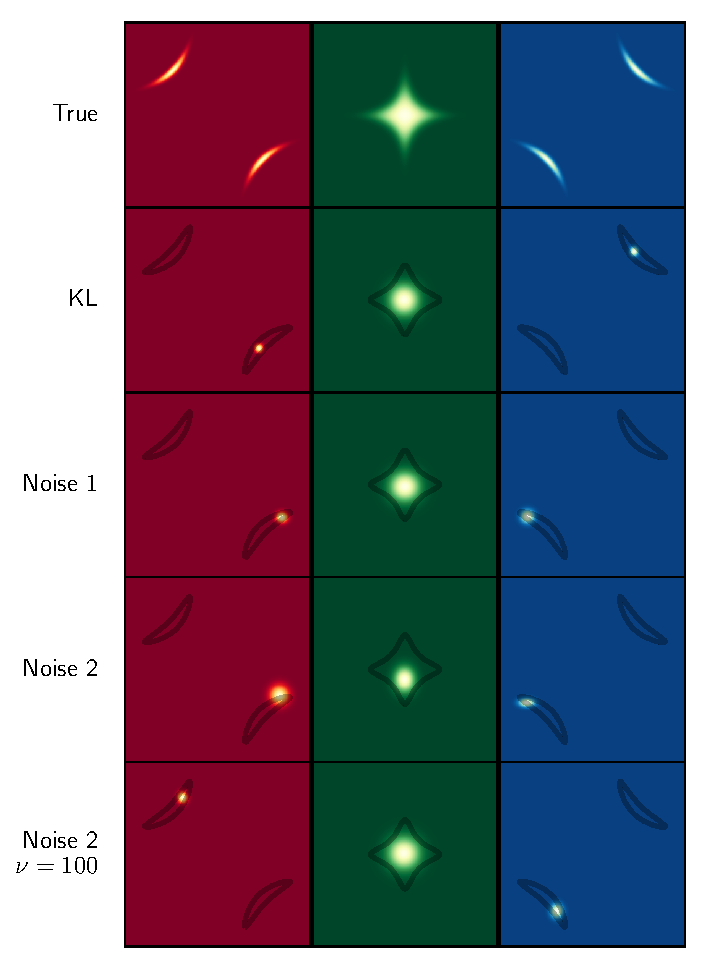
\includegraphics[]{landmark-posteriors-gaussian-model.png}
  \captionof{figure}{The top 4 plots show the marginals of the model, along with two different choices of noise in VNCE. The next row of 3 plots show $p(\z | \x_i)$ for 3 different colour-coded landmark $\x_i$ points, whose location can be read-off from the plot of $p(\x)$. The subsequent rows correspond to different approximate posteriors for each of the landmark points: the first learnt using standard variational inference with the KL-divergence, and the last 3 using VNCE.}
  \label{fig:posterior visualisation}
\end{minipage}
    \clearpage
}

The ground-truth row in figure \ref{fig:posterior visualisation} illustrates how a relatively simple model can generate complex posteriors that vary greatly depending on which $\x$ we condition on. For some $\x$ we generate relatively well-behaved, uni-modal posteriors resembling a laplacian (green), whilst for other $\x$, we generate multi-modal posteriors concentrated along curved manifolds (blue \& red). Fitting an approximate posterior to such diverse distributions is challenging, which is why a highly expressive function approximator such as a neural network is needed. Even with a neural network, our current parameterisation restricts us to outputting a Gaussian with diagonal covariance, which is a poor match for any of the true posteriors.

We see that the approximate posterior learnt by minimising the KL-divergence is `mode-seeking', latching onto a single density peak, whilst \emph{underestimating} the variance of this peak. This behaviour is well-known and predictable from the mathematical form of the KL:
\begin{align}
    \infdiv{KL}{q(\z \given \x ; \alphab)}{p(\z \given\x)} = \Evar{\x} \left[ \log \frac{q(\z \given \x ; \alphab)}{p(\z \given\x)}\right],
\end{align}
since if $q$ places any probability mass in a region where $p$ is unlikely, then the denominator in the log is close to zero, exploding the KL.

Of greater interest to us is the fact that approximate posteriors learnt with VNCE display similar low-variance, mode-seeking behaviour. The key difference with VNCE is that the choice of noise distribution and ratio of noise-to-data samples, $\nu$, affect the shape of the posteriors. When the noise is `good’ and roughly resembles the data, or when $\nu$ is appropriately large, we obtain posteriors resembling those produced by the ELBO - see rows 3 & 5 of fig \ref{fig:posterior visualisation}. However, when the noise does not resemble the data and nu is small, we obtain warped posteriors that, visually, are worse matches to the true posterior - see row 4.

The results here validate lemma \ref{lemma: diff J - J1}, which stated the f-divergence between the approximate and true posterior that we minimise in VNCE. In particular, corollary \ref{corollary: f-divergence limit}, which directly followed from the lemma, showed that this f-divergence tends towards the KL when $\pnn(\x)/(\pnn(\x) + \nu \pnoise(\x)) \rightarrow 0$. That is, when the noise assigns a high density to $\x$ compared to the model, or when $\nu$ is large, we expect VNCE to produce a similar posterior to the ELBO at that \emph{specific} point $\x$. We see this in practice: noise 1 assigns a high density to the green landmark, and so the posterior resembles that of the KL here. The same is true of noise 2 when $\nu=100$, but \emph{not} when $\nu=1$, since noise 2 is very diffuse and assigns a low density to this point compared to the model. All three setting of VNCE produce posteriors that are slightly different to the KL at the extreme red and blue landmarks. This is because neither noise is a good match to the model here, and whilst increasing $\nu$ helps, it does not entirely fix the issue. Even though the VNCE posteriors do not always match the KL posteriors, when the noise is good and/or when $\nu$ is large, we obtain reasonable approximations to the true posteriors (modulo the restrictive parametric assumptions).

\subsection{A toy problem for visualising parameter estimation with VNCE}
\label{sec:mog}
We consider a simple mixture of two Gaussians model, where the only unknown parameter is the standard deviation of one of the Gaussians. We consider two cases: firstly a normalised MoG, and then an unnormalised version. Finally, for the unnormalised version, we run a population analysis to compare the performance of VNCE against both NCE and maximum likelihood estimation across multiple sample sizes.

%%%%%%%%%%%%%%%%%%%%%%%%%%%%%%%%%%%%%%%%%%%%%%%%%%%%%%%%%%%%%%%%%%%%%%%%%%%%%%%%%%%%%%%%%%%%%%%%%%%%%%%%%%%%%%%%%%%%%
%                                        NORMALISED MIXTURE OF GAUSSIANS
%%%%%%%%%%%%%%%%%%%%%%%%%%%%%%%%%%%%%%%%%%%%%%%%%%%%%%%%%%%%%%%%%%%%%%%%%%%%%%%%%%%%%%%%%%%%%%%%%%%%%%%%%%%%%%%%%%%%%

\subsubsection{Normalised Mixture of Gaussians}

%\begin{figure}[ht]
%  \centering
%  \includegraphics[scale=0.4]{em-loss-curve-mog.pdf}
%    \caption{\label{fig:mog-em-loss-curve} EM type algorithm applied to a normalised Mixture of Gaussians %model. The red lines indicate when we make the update $q(z|u) = p(z|u; \theta_k)$ where $\theta_k$ is the %value of $\theta$ at that point during the optimisation.}.
%\end{figure}

\noindent A common latent variable model is the Mixture of Gaussian (MoG) model. For a mixture with two components, a single binary latent variable $z \sim \mathcal{B}er(\pi)$ determines which of two Gaussians the data was generated from. if $\pi = 1/2$, we have the following joint:
\begin{equation}
\pnorm(u, z; \theta) = \frac{(1-z)}{2} \mathcal{N}(u; 0, \theta) + \frac{z}{2} \mathcal{N}(u; 0, \sigma_1).
\label{eq:mog standard}
\end{equation}
We assume that the variance of the second component, $\sigma_1^2$, is known, and our task is to estimate the value of $\theta$. Whilst this estimation problem does not involve an unnormalised model, we can still apply VNCE to it. This provides a useful sanity check of the method's validity in a simple setting where we do not have a scaling parameter to estimate in conjunction with $\theta$.

For a simple experiment, we set $\sigma_1 = 1$ and let $\theta^* = 4$ be the true value of $\theta$. We then make the following choices of noise and variational distribution:
\begin{align}
    \label{eq:normalised mog posterior}
    \pnoise(u) &= \mathcal{N}(u; 0, \theta^*) \\
    q(z|u) &= p(z=0 \ | \ u; \theta) = \left(  1 + \frac{\theta_k}{\sigma_1} \exp \left(\frac{- u^2}{2} \left( \frac{1}{\sigma_1^2} - \frac{1}{\theta^2} \right) \right) \right)^{-1}.
\end{align}
The choice of noise distribution is not too important for this simple model, so long as it very approximately matches the data generating distribution. With this setup, we can then apply the EM type algorithm discussed in section \ref{sec:optimisation of var objective}. We can visualise this algorithm by iteratively plotting the variational bound, for all values of $\theta$, each time we update the variational distribution $q$ in figure \ref{fig:normalised-mog}. It is clear from the figure that the algorithm converges to the correct value of $\theta$.

\afterpage{
    \thispagestyle{empty}
    \begin{figure}[ht]
      \centering
      \caption{\label{fig:normalised-mog} EM type algorithm applied to a normalised Mixture of Gaussians model. The notation $J^1_{\theta_k}$ in the legends refers to the variational lower bound of the NCE objective function where the variational distribution $q(z|u)$ is set to $p(z|u; \theta_k)$}.
      \includegraphics[width = 0.9 \textwidth]{variational-em.pdf}
    \end{figure}
    \clearpage
}

%%%%%%%%%%%%%%%%%%%%%%%%%%%%%%%%%%%%%%%%%%%%%%%%%%%%%%%%%%%%%%%%%%%%%%%%%%%%%%%%%%%%%%%%%%%%%%%%%%%%%%%%%%%%%%%%%%%%%
%                                        UNNORMALISED MIXTURE OF GAUSSIANS
%%%%%%%%%%%%%%%%%%%%%%%%%%%%%%%%%%%%%%%%%%%%%%%%%%%%%%%%%%%%%%%%%%%%%%%%%%%%%%%%%%%%%%%%%%%%%%%%%%%%%%%%%%%%%%%%%%%%%

\subsubsection{Unnormalised Mixture of Gaussians}

\noindent We would like to modify the MoG given in equation \ref{eq:mog standard} to obtain an unnormalised family. An obvious candidate is:
\begin{equation}
\phi(u, z; \theta, c) = e^{-c} \left( (1-z) e^{-\frac{u^2}{2 \theta^2}} + z e^{-\frac{u^2}{2 \sigma_1^2}} \right)
\label{eq:mog unnormalised}
\end{equation}
where $e^{-c}$ is a scaling parameter needed for NCE, as discussed at the end of section \ref{sec:nce}. It is important to note that the usual MoG family in equation \ref{eq:mog standard} is \emph{not} nested within unnormalised family in equation \ref{eq:mog unnormalised}. We can see this more easily by normalising \ref{eq:mog unnormalised}, giving us:
\begin{equation}
    \pnorm(u, z, \theta) = (1-z)\frac{\theta}{\theta + \sigma_1} \mathcal{N}(u; 0, \theta) +
                     z\frac{\sigma_1}{\theta + \sigma_1} \mathcal{N}(u; 0, \sigma_1)
\label{eq:mog normalised version of unnormalised}
\end{equation}
We see that the parameter $\theta$ of the unnormalised MoG controls both the width of the first component and its scale relative to the second component. 

As before, fix $\sigma_1 = 1$ and $\theta^*=4$. Using equation \ref{eq:mog normalised version of unnormalised}, we can easily sample synthetic data from our unnormalised model $\phi$ (still under the assumption that $z \sim \mathcal{B}er(\frac{1}{2})$). To do so, we simply sample $w \sim \mathcal{B}er(\frac{\sigma_1}{\theta + \sigma_1})$ and then sample $\{x_1, ..., x_i\}$ data points:
\[
    x_i \sim \left\{\begin{array}{lr}
        \mathcal{N}(u; 0, \theta), & \text{if } w = 0\\
         \mathcal{N}(u; 0, \sigma_1), & \text{if } w = 1
        \end{array}
\]
Using this synthetic data, we can proceed as before, using an EM algorithm to learn the parameter $\theta$. To do this, we would need to use the posterior over latents, given by:
\begin{equation}
    p(z=0 \ | \ u) = \frac{1}{1 + \exp(\frac{-u^2}{2} (\frac{1}{\sigma_1^2} + \frac{1}{\sigma_0^2}) )}.
\end{equation}
However, for more complex models, we do not have access to such a posterior, and so it is important that VNCE still works when we approximate it with a parametrised variational distribution $q$. To test this, we use the following $q$:
\begin{equation}
    q(z=0 \ | \ u; \textbf{w}) = \frac{1}{1 + \exp(w_0 + w_1u + w_2u^2)}, 
\end{equation}
which clearly contains the true posterior.

Visualising learning is less straightforward now that our parameter set is 2-dimensional, but we can compare the contour plot of the true NCE objective function against the lower bound obtained at the end of learning. This is given in figure \ref{fig:unnormalised mog contour}. We see that the algorithm converges to the correct value of $\theta$, and correct normalising constant.

\afterpage{
    \thispagestyle{empty}
    \begin{figure}[ht]
    \centering
    \includegraphics[width = 0.8 \textwidth]{unnormalised-mog-countour.pdf}
    \vspace*{-18mm}
    \caption{\label{fig:unnormalised mog contour} Contour plot of true NCE objective function compared to the variational lower bound for an unnormalised Mixture of Gaussians. For the lower bound, we have set the variational distribution $q(z|u)$ to be the posterior $p(z|u; \tilde{\theta})$, where $\tilde{\theta}$ is our final estimate obtained after optimisation. The vertical axis corresponds to $c$, the scaling parameter.}
    \end{figure}
    \clearpage
}

%%%%%%%%%%%%%%%%%%%%%%%%%%%%%%%%%%%%%%%%%%%%%%%%%%%%%%%%%%%%%%%%%%%%%%%%%%%%%%%%%%%%%%%%%%%%%%%%%%%%%%%%%%%%%%%%%%%%%
%                                       MOG POPULATION ANALYSIS
%%%%%%%%%%%%%%%%%%%%%%%%%%%%%%%%%%%%%%%%%%%%%%%%%%%%%%%%%%%%%%%%%%%%%%%%%%%%%%%%%%%%%%%%%%%%%%%%%%%%%%%%%%%%%%%%%%%%%
\subsubsection{Population Analysis of unnormalised Mixture of Gaussian model}

Figure \ref{fig:mse-mog} shows the MSE $\mathbb{E} ||\theta - \theta^*||^2$ for VNCE, NCE and maximum likelihood across multiple runs and with different sample sizes. To produce it, we generated 500 distinct ground-truth values for standard deviation parameter in the unnormalised MoG, sampling uniformly from the interval $[2, 6]$. For each of the 500 $\theta^*$s, we estimate it using all three estimation methods and with a range of sample sizes. Every run was initialised from five random values and the best result out of the five was kept in order to avoid local optima, which exist since both the likelihood and NCE objective functions are bi-modal.

Figure \ref{fig:mse-mog} (a) demonstrates that the estimation accuracy of VNCE increases with sample size, and is comparable to that of NCE. This gives some evidence of the consistency of VNCE. We note that the comparison is complicated by the fact that NCE was particularly prone to falling into local optima (despite our use of multiple random initialisations). This is why NCE's worst-case accuracy is significantly worse than that of the other two methods, as shown by the upper dashed blue line.

\begin{figure}[t]
\centering
\begin{subfigure}{.5\textwidth}
  \centering
  \includegraphics[width=1.1\linewidth]{sample-size-against-mse.pdf}
  \caption{Standard deviation}
  \label{fig:sub1}
\end{subfigure}%
\begin{subfigure}{.5\textwidth}
  \centering
  \includegraphics[width=1.1\linewidth]{sample-size-against-mse-scaling-param.pdf}
  \caption{Scaling parameter}
  \label{fig:sub2}
\end{subfigure}
\caption{log sample size against log mean-squared error (MSE) produced when estimating the standard deviation and scaling parameter for 500 different unnormalised Mixture of Gaussian models. The thick central lines show the median MSE of the 500 runs, whilst the dashed lines mark the 1st and 9th deciles. The constant negative slope of the red line is evidence of the consistency of VNCE.}
\label{fig:mse-mog}
\end{figure}

%%%%%%%%%%%%%%%%%%%%%%%%%%%%%%%%%%%%%%%%%%%%%%%%%%%%%%%%%%%%%%%%%%%%%%%%%%%%%%%%%%%%%%%%%%%%%%%%%%%%%%%%%%%%%%%%%%%%%
%                                        RESTRICTED BOLTZMANN MACHINES
%%%%%%%%%%%%%%%%%%%%%%%%%%%%%%%%%%%%%%%%%%%%%%%%%%%%%%%%%%%%%%%%%%%%%%%%%%%%%%%%%%%%%%%%%%%%%%%%%%%%%%%%%%%%%%%%%%%%%
\subsection{Restricted Boltzmann Machine}
\label{sec:rbm}

The Restricted Boltzmann Machine (RBM) \citep{smolensky1986information} is an unnormalised, latent variable model over binary vectors given by:
\begin{align}
p(\u, \z, ; \thetab)  \propto \exp(\u^TW\z + \textbf{a}^{T}\u + \textbf{b}^T\z) \ ,
\label{eq:rbm}
\end{align}
where $W \in \mathbb{R}^{d \times m}$; $\textbf{a}, \u \in \mathbb{R}^{d}$; $\textbf{b}, \z \in \mathbb{R}^{m}$, and $\thetab \equiv (W, \textbf{a}, \textbf{b})$. We refer to $W$ as the weight matrix and $\textbf{a}$ and $\textbf{b}$ as the biases. $\u$ contains the visible variables/units and $\z$ the hidden units, which are typically of lower dimension since we would like to find a smaller set of random variables that capture the correlations between the higher-dimensional observations.

\begin{figure}[!h]
\centering
% Adapted from: https://github.com/MartinThoma/LaTeX-examples/blob/master/tikz/restricted-boltzmann-machine/restricted-botzmann-machine.tex
\begin{tikzpicture}[scale=2]
    % \draw ;
    \draw[fill=black!30, rounded corners] (-0.2, -0.2) rectangle (3.2, 0.2) {};
    \draw[fill=black!30, rounded corners] (0.3, 0.8) rectangle (2.7, 1.2) {};

    \node (u1)[neuron] at (0, 0) {$u_1$};
    \node (u2)[neuron] at (1, 0) {$u_2$};
    \node (u3)[neuron] at (2, 0) {$u_3$};
    \node (u4)[neuron] at (3, 0) {$u_4$};
    \node[right=0.1cm of u4] (u) {$\textbf{u} \in \{0, 1\}^4$};
    \node[learned,below=0.1cm of u1] (a1) {$a_{1}$};
    \node[learned,below=0.1cm of u2] (a2) {$a_{2}$};
    \node[learned,below=0.1cm of u3] (a3) {$a_{3}$};
    \node[learned,below=0.1cm of u4] (a4) {$a_{4}$};

    \node (z1)[neuron] at (0.5, 1) {$z_1$};
    \node (z2)[neuron] at (1.5, 1) {$z_2$};
    \node (z3)[neuron] at (2.5, 1) {$z_3$};
    \node[right=0.1cm of z3] (z) {$\textbf{z} \in \{0, 1\}^3$};
    \node[learned,above=0.1cm of z1] (b1) {$b_{1}$};
    \node[learned,above=0.1cm of z2] (b2) {$b_{2}$};
    \node[learned,above=0.1cm of z3] (b3) {$b_{3}$};

    \node[learned] (W) at (3.5, 0.5) {$W \in \mathbb{R}^{3 \times 4}$};

    \draw[learned,stateTransition] (u1) -- (z1) node [midway,above=-0.06cm,sloped] {$w_{1,1}$};
    \draw[stateTransition] (u1) -- (z2) node [midway,above=-0.06cm,sloped] {};
    \draw[stateTransition] (u1) -- (z3) node [midway,above=-0.06cm,sloped] {};

    \draw[stateTransition] (u2) -- (z1) node [midway,above=-0.06cm,sloped] {};
    \draw[stateTransition] (u2) -- (z2) node [midway,above=-0.06cm,sloped] {};
    \draw[stateTransition] (u2) -- (z3) node [midway,above=-0.06cm,sloped] {};

    \draw[stateTransition] (u3) -- (z1) node [midway,above=-0.06cm,sloped] {};
    \draw[stateTransition] (u3) -- (z2) node [midway,above=-0.06cm,sloped] {};
    \draw[stateTransition] (u3) -- (z3) node [midway,above=-0.06cm,sloped] {};

    \draw[stateTransition] (u4) -- (z1) node [midway,above=-0.06cm,sloped] {};
    \draw[stateTransition] (u4) -- (z2) node [midway,above=-0.06cm,sloped] {};
    \draw[learned,stateTransition] (u4) -- (z3) node [midway,above=-0.06cm,sloped] {$w_{4,3}$};

\end{tikzpicture}
\caption{The undirected graph for a Restricted Boltzmann Machine.}
\label{fig:rbm-graph}
\end{figure}

In order to see how the hidden units in an RBM explain the couplings between the visible units, it helps to picture an undirected graph over which the model factorizes as in figure \ref{fig:rbm-graph}. Note that the Markov blanket of each $u_i$ is $\z$, and, conversely, the Markov blanket of each $z_i$ is $\u$. Therefore, we obtain the factorisations:
\begin{equation}
    p(\u | \z) = \prod_{i=1}^d p(u_i | \z)  \ \ \ \ \ \ \ p(\z \given \u) = \prod_{i=1}^m p(z_i | \u) \ ;
    \label{eq: rbm conditional indpendicies}
\end{equation}
the first factorisation says that the visible units are independent given the latents and thus the latents capture correlations in the visibles.

We gain further insight into the model's properties by not only considering it's conditional independencies, but its specific parametric form, as given in equation \ref{eq:rbm}. If we marginalise out the latent variables, we obtain:
\begin{align}
    p(\u) &= \sum_{z_1, ..., z_m} p(\u, \z) \\
          &\propto \exp(\textbf{a}^T\u) \prod_{i=1}^m \sum_{z_i \in \{0, 1\}} \exp(b_i z_i + z_i \u^T W_{:, i}) \\
          &\propto \exp(\textbf{a}^T\u) \prod_{i=1}^m (1 + \exp(b_i + \u^T W_{:, i})) \ ,
          \label{eq:marginal of rbm}
\end{align}
where $W_{:, i}$ is the $i^{th}$ column of the weight matrix $W$. Since $p(\u)$ is a product over $m+1$ terms, we can think of the RBM as a `product of experts' \citep{hinton2006training}:
\begin{equation}
    p(\u) \propto \prod_{i=1}^{m+1} f_i(\u)
\end{equation}
where each expert `votes' on the probability of a vector $\u$. Since the experts act multiplicatively, the resulting distribution can be quite sharp, since each expert can vote for a specific sub-region of the input space. In the RBM, each expert takes the inner product of a fixed `template' vector --- $W_{:,i}$ or $\textbf{a}$ --- with the input $\u$, and so inputs that match multiple templates are likely under the model.

%%%%%%%%%%%%%%%%%%%%%%%%%%%%%%%%%%%%%%%%%%%%%%%%%%%%%%%%%%%%%%%%%%%%%%%%%%%%%%%%%%%%%%%%%%%%%%%%%%%%%%%%%%%%%%%%%%%%%
%                                         TRAINING RBMS
%%%%%%%%%%%%%%%%%%%%%%%%%%%%%%%%%%%%%%%%%%%%%%%%%%%%%%%%%%%%%%%%%%%%%%%%%%%%%%%%%%%%%%%%%%%%%%%%%%%%%%%%%%%%%%%%%%%%%

\subsubsection{Training Restricted Boltzmann Machines}
\label{sec:training_rbms}

The factorisation of p(\u) in equation \ref{eq:marginal of rbm} shows that marginalising out the latents is cheap for an RBM, costing only $O(m)$ time, where $m$ is the dimension of the latent vector $\z$. However, computing the partition function \emph{is} intractable, since we would have to compute:
\begin{align}
    Z(\thetab) = \sum_{\u \in \{0, 1\}^d} \exp(\textbf{a}^T\u) \prod_{i=1}^m (1 + \exp(b_i + \u^T W_{:, i})) \ ,
\end{align}
which cannot be further factorised due to the presence of $\u$ in every term of the product. Naively, computing $Z(\thetab)$ costs $O(m2^d)$. We can rearrange the sums to reduce this to $O(d2^m)$, but this is still exponential in the number of hidden units. Further optimisations exist to reduce the cost, but it is still infeasible to compute for much more than around 30 hidden units. 

Hence, we are not dealing with the general case that VNCE was designed for: when \emph{both} marginalising out the hiddens and computing the partition function are intractable. Since only the latter is intractable, we can apply NCE to the problem. As with the mixture of Gaussians, this is useful since we can compare the performance of NCE to VNCE.

Another important comparison to make is with contrastive divergence since it is perhaps the most common method for training an RBM. As discussed in section \ref{sec:cd}, contrastive divergence roughly approximates the gradient ascent rule for maximum likelihood learning, using updates of the form:
\begin{align}
    \label{eq:cd grad update for rbm}
    \nabla_{W} \ell(\thetab) &= \Edata \E_{\z \sim p(\z \given \x)} \left[ \nabla_{W} \log \pnn(\x, \z;\thetab) \right] - \E_{\x, \z \sim p_k(\x, \z)} \left[\nabla_{W} \log \left(\pnn(\x, \z;\thetab) \right) \right] \\
                      &= \Edata \E_{\z \sim p(\z \given \x)} \left[ u_i z_j \right] - \E_{\x, \z \sim p_k(\x, \z)} \left[ u_i z_j \right] \ ,
\end{align}
for the weight matrix $W$ (similar updates are used for the biases). The notation $p_k$ refers to the distribution obtained after running a Markov Chain Monte Carlo method for $k$ steps, starting at the data generating distribution $p^*$. If we took $k \rightarrow \infty$, then we would obtain $p$ (the current model). Whilst we are free to choose amy MCMC method, in the case of an RBM, the conditional independence statements in equation \ref{eq: rbm conditional indpendicies} allow us to implement efficient block-Gibbs sampling, where we alternate between sampling $\u | \z$ and $\z \given \u$.

To our knowledge, there is no prior work comparing NCE to contrastive divergence in the case of the RBM, so the following experiments consider all three pairwise comparisons of VNCE, NCE and contrastive divergence.


%%%%%%%%%%%%%%%%%%%%%%%%%%%%%%%%%%%%%%%%%%%%%%%%%%%%%%%%%%%%%%%%%%%%%%%%%%%%%%%%%%%%%%%%%%%%%%%%%%%%%%%%%%%%%%%%%%%%%
%                                        RBM EXPERIMENTAL SETUP
%%%%%%%%%%%%%%%%%%%%%%%%%%%%%%%%%%%%%%%%%%%%%%%%%%%%%%%%%%%%%%%%%%%%%%%%%%%%%%%%%%%%%%%%%%%%%%%%%%%%%%%%%%%%%%%%%%%%%

\subsubsection{Experimental Setup}

Following \citet{carreira2005contrastive}, we use a toy dataset derived from all mutually exclusive $3 \times 3$ patches of the 11,000 $16 \times 16$ images of handwritten digits from the USPS dataset.\footnote{https://cs.nyu.edu/~roweis/data.html} After thresholding the 256 intensity levels at 150, we obtained 275,000 9-dimensional binary vectors. We use this relatively low-dimensional toy dataset in order to make computing the partition function, and hence the log-likelihood, cheap.

For all three estimation methods, we train RBMs with varying number of hidden units: $m \in \{2, 4, 6, 8\}$. For each value of $m$, we use the same initial weights and biases across all three methods, sampling the weights and hidden biases with: $W_{i, j} \sim \mathcal{U}(-4 \sqrt{\frac{6}{d + m}}, 4 \sqrt{\frac{6}{d + m})$ and setting the visible biases to $\frac{\log(p_i)}{1 - \log(p_i)}$ where $p_i$ is the empirical frequency of $u_i = 1$. Setting the visible biases in this way ensures that the initial model approximately matches the empirical marginals, and hence most of training consists in discovering the correlations between the visibles. For VNCE and NCE we must also initialise the scaling parameter; we set it to $-m \log(2) + \sum_{i=0}^{d}(\log(1 - p_i))$, which approximately normalises the initial model (it would exactly normalise it if the weight matrix and hidden biases were initialised to zero).

For contrastive divergence, we use the largest stable learning rate, which is 0.1, a batch size of 100 and train for 100 epochs. For each data point in a batch, we initialise a Markov chain at that point and run it for 1 step to produce 100 `fantasy' samples. Many implementations of CD \citep{hinton2012practical} do not actually take samples of the latent variables on the \emph{final} step of Gibbs sampling. Instead they directly use the probability of the latents to compute the gradient update. Whilst this is a useful property of CD in the case of the RBM, for many other models we will be forced to take samples. Hence, to make our comparison of VNCE and CD fair for the general case, we always take samples.

For both VNCE and NCE, we set the noise distribution over visible units to be a product of marginals. Each marginal is a Bernoulli distribution, with parameter $p_i$ equal to the empirical marginal probability. We set the ratio of noise to data samples, $\nu$, equal to 1. We optimise their objective functions using stochastic gradient ascent (SGD) with the same settings as for contrastive divergence. We also investigated using a non-linear optimiser such as L-BFGS-B, however they tend not to scale well to large datasets. In addition, when using VNCE with L-BFGS-B inside the inner loop of the EM-algorithm, we have found that waiting for the built-in convergence criterion causes slow overall convergence. This can be remedied however by limiting the number of iterations to a small number rather than waiting for convergence.

For VNCE, we update the variational distribution $q$ to equal the model's current posterior over latents at every E-step of the EM algorithm. In the general case $q$ will have its own parameters but for the RBM this is not necessary since we have an analytic expression for $p(\z \given \u)$ given in equation \ref{eq: rbm conditional indpendicies} that is efficient to sample from.

%%%%%%%%%%%%%%%%%%%%%%%%%%%%%%%%%%%%%%%%%%%%%%%%%%%%%%%%%%%%%%%%%%%%%%%%%%%%%%%%%%%%%%%%%%%%%%%%%%%%%%%%%%%%%%%%%%%%%
%                                         RBM EXPERIMENTAL RESULTS
%%%%%%%%%%%%%%%%%%%%%%%%%%%%%%%%%%%%%%%%%%%%%%%%%%%%%%%%%%%%%%%%%%%%%%%%%%%%%%%%%%%%%%%%%%%%%%%%%%%%%%%%%%%%%%%%%%%%%

\subsubsection{Experimental Results}

\afterpage{
    \thispagestyle{empty}
\noindent\begin{minipage}[h]{\textwidth}
%   \vspace*{\fill}
  \centering
  \includegraphics[scale=0.8]{usps-different_num_hiddens.png}
  \noindent
  \centering
  \includegraphics[scale=0.8]{usps-different_num_hiddens-4by-4.png}
  \captionof{figure}{Learning curves for CD, NCE and VNCE when training Restricted Boltzmann Machines on binarised image patches with the number of hidden units in $\{2, 4, 6, 8\}$. The top 4 plots are for $3 \times 3$ patches, whilst the lower 4 plots are for $4 \times 4$ patches. All models here were trained with SGD. The green dashed line is the log-likelihood of the noise distribution used in NCE, which in this case is a product of the empirical marginals.}
  \label{fig:usps-rbm-4by4}
\end{minipage}
    \clearpage
}
Figure \ref{fig:usps-rbm-4by4} shows the learning curves for training RBMs with SGD using a range of latent dimensions: $m \in \{2, 4, 6, 8\}$. In all cases, we see contrastive divergence converges to a higher log-likelihood than NCE or VNCE, although the gap in final log-likelihoods is very small for $m=2$ hidden units, and grows with $m$. NCE and VNCE converge to the same final log-likelihood, showing that the variational approximation has not compromised the quality of the final model. The estimation methods differ significantly in terms of speed: The log-likelihood reached by VNCE at convergence is obtained 2-5x more quickly by NCE, and 10-50x more quickly by contrastive divergence. We note that the final gap between NCE/VNCE and contrastive divergence could be narrowed with a more sophisticated choice of noise distribution or by using a larger ratio of noise to data samples, at the cost of speed.

These results are strongly in favour of contrastive divergence as a method for training RBMs, particularly as we increase the number of hidden units. This observation is consistent with the limited theory that exists for contrastive divergence. As discussed in section \ref{sec:cd}, the difference between the maximum likelihood gradient updates and contrastive divergence updates as stated in equation \ref{eq:cd bias}, can be analytically bounded in the case of the RBM. \citet{bengio2009justifying} provided a bound, later improved by \citet{fischer2011bounding}, which was demonstrated to be both tight and small on a toy problem. More generally the authors show that the bound will be small when the absolute values of the RBM parameters are small. This theory gives us some assurance that contrastive divergence will work well for the RBM, and the theory appears to borne out in practice.

Nevertheless, the amount of bias in contrastive divergence learning can be much larger for particular data generating distributions \citep{marlin2010inductive}, and may be larger for other classes of models. In particular, one might expect that for models where MCMC sampling is less efficient (because we cannot do block sampling, say), that contrastive divergence will be less effective. We investigate these possibilities in subsequent experiments.


%%%%%%%%%%%%%%%%%%%%%%%%%%%%%%%%%%%%%%%%%%%%%%%%%%%%%%%%%%%%%%%%%%%%%%%%%%%%%%%%%%%%%%%%%%%%%%%%%%%%%%%%%%%%%%%%%%%%%
%                                        SELF-CONTRASTIVE VNCE
%%%%%%%%%%%%%%%%%%%%%%%%%%%%%%%%%%%%%%%%%%%%%%%%%%%%%%%%%%%%%%%%%%%%%%%%%%%%%%%%%%%%%%%%%%%%%%%%%%%%%%%%%%%%%%%%%%%%%
\newpage
\section{Adaptive VNCE}
\citet{goodfellow2014distinguishability} proposed a variation of NCE where, after each update of the parameters $\thetab$, we reset the noise distribution to be equal to the current model. He showed that this scheme, termed `self-contrastive estimation', yields the same gradient updates as maximum likelihood learning. We prove an analog of this result for the latent-variable case, and investigate how to efficiently implement it.

In the the appendix, section \ref{sec:appendix grad of J1}, we derive the gradient of the VNCE objective function, which is:
\begin{align}
\nabla_{\theta}J_1(\theta) & =  
        \Ex \mathbb{E}_{\z \sim q} \left[ \frac{\nu}{r(\x, \z ; \thetab) + \nu}
        \gradtheta \log(\phi(\x, \z; \thetab)) \right] \\
    & - \Ey
        \frac{\nu}{\mathbb{E}_{\z \sim q}[r(\y, \z; \thetab)] + \nu}
        \mathbb{E}_{\z \sim q} \left[ r(\y, \z; \theta) \gradtheta \log(\phi(\y, \z; \thetab)) \right]
\end{align}
where,
\begin{equation}
    r(\u, \z; \theta) = \frac{\pnn(\x, \z ; \thetab)}{q(\z \given \u) \pnoise(\u)}
\end{equation}
Now let us suppose that during each E step, not only do we set $q_k(\z \given \u) = p(\z \given \u; \thetab_k)$, but we also update the noise to be equal to the current model over visibles: $\pnoise(\u) = \pnn(\u; \thetab_k)$. Then,
\begin{equation}
     r(\u, \z; \theta) = \frac{\pnn(\x, \z ; \thetab)}{p(\z \given \u; \thetab_k)  \pnn(\u; \thetab_k)} = 1 \ ,
\end{equation}
which implies that the gradient is:
\begin{equation}
    \label{eq:self-contrastive vnce is mle}
    \nabla_{\theta}J_1(\theta) & =  \frac{\nu}{1 + \nu} \Big(
       \Ex \Evar{\x} \left[ \gradtheta \log(\phi(\x, \z; \thetab)) \right]
     - \Ey \Evar{\y}  \left[ \gradtheta \log(\phi(\y, \z; \thetab)) \right] \Big) \ ,
\end{equation}
which is proportional to the maximum likelihood gradient update, as presented in equation \ref{eq:unnormalised latent var mle gradient} in section \ref{sec:mle}.

Now, if during the M-step we only take a single gradient step using equation \ref{eq:self-contrastive vnce is mle}, and then repeat the E-step as stated above, then we have precisely recovered maximum likelihood estimation. If however, we take multiple gradient steps during the M-step, we have a new adaptive version of VNCE that approximates maximum likelihood learning, but is potentially faster. The main problem with this adaptive scheme is that at each E-step, we must acquire noise samples from $\pnn(\u; \thetab_k)$, which could be costly if we have to run an Markov chain Monte Carlo method for a long time. This is the same problem faced by maximum likelihood learning, and one solution there is to only run the Markov chain for $k$ steps, initialising it at a data point. In other words, we can use \emph{contrastive divergence}.

Hence, we have developed an adaptive version of VNCE that includes maximum likelihood and contrastive divergence as special cases. The main question of interest is whether deviating from these special cases, by using multiple gradient updates during the M-step of learning, leads to a faster or more accurate learning method.

%%%%%%%%%%%%%%%%%%%%%%%%%%%%%%%%%%%%%%%%%%%%%%%%%%%%%%%%%%%%%%%%%%%%%%%%%%%%%%%%%%%%%%%%%%%%%%%%%%%%%%%%%%%%%%%%%%%%%
%                                        VNCE WITH LATENT VARIABLE NOISE
%%%%%%%%%%%%%%%%%%%%%%%%%%%%%%%%%%%%%%%%%%%%%%%%%%%%%%%%%%%%%%%%%%%%%%%%%%%%%%%%%%%%%%%%%%%%%%%%%%%%%%%%%%%%%%%%%%%%%
\section{VNCE with Latent Variable Noise}
\label{sec:vnce with latent variable noise}
We have shown in section \ref{sec:VNCE} that one can obtain a variational lower bound to the first term of the NCE objective function:
\begin{align}
\label{eq:vnce with latent noise lower bound 1}
    \color{red}{\Ex  \log \left(\frac{\int \pnn(\x, \z;\thetab) \dif \z}{\int \pnn(\x, \z;\thetab) \dif \z + \nu \pnoise(\x)}\right)}
    \geq  \color{red}{\Ex \mathbb{E}_{q_1(\z \given \x)} \log \left( \frac{\pnn(\x,\z; \thetab)}{\pnn(\x,\z; \thetab) + \nu q_1(\z \givenx)\pnoise(\x)} \right)}
\end{align}
However, because of the symmetry in the NCE objective function, we can apply the same inequality to the second term under the assumption that our noise has latent variables:
\begin{align}
\label{eq:vnce with latent noise lower bound 2}
    \color{blue}{\nu \Ey  \log \left(\frac{ \nu \int \pnoise(\y, \z) \dif \z}{\nu \int \pnoise(\y, \z) \dif \z + \pnn(\x ; \thetab)} \right)}
    \geq  \color{blue}{ \nu \Ey \mathbb{E}_{q_2(\z \given \y)} \log \left( \frac{\nu \pnoise(\y, \z))}{\nu \pnoise(\y, \z) +  q_2(\z \given \y) \pnn(\y ; \thetab) } \right)}.
\end{align}
Where $q_2$ is a second variational distribution that is potentially distinct from $q_1$. Observe that the first inequality (\ref{eq:vnce with latent noise lower bound 1}) contains the term: $\pnoise(\x)$, whilst the second inequality (\ref{eq:vnce with latent noise lower bound 2}) contains the term $\pnn(\y; \thetab)$. Both of these terms depend on latent variables and are assumed to be intractable. The way we have currently dealt with this problem is to use importance sampling, which would give us:
\begin{align}
\label{eq:variational noise, term 1 with importance sampling}
    \color{red}{\Ex \mathbb{E}_{q_1(\z \given \x)} \log \left( \frac{\pnn(\x,\z; \thetab)}{\pnn(\x,\z; \thetab) + \nu q_1(\z \given \x) \mathbb{E}_{q_2(\z \given \x)} \left[ \frac{\pnoise(\x, \z)}{q_2(\z \given \x)} \right]} \right)}
\end{align}
and 
\begin{align}
\label{eq:variational noise, term 2 with importance sampling}
    \color{blue}{ \nu \Ey \mathbb{E}_{q_2(\z \given \y)} \log \left( \frac{\nu \pnoise(\y, \z))}{\nu \pnoise(\y, \z) +  q_2(\z \given \y) \mathbb{E}_{q_1(\z \given \y)}\left[ \frac{\pnn(\y , \z; \thetab)}{q_1(\z \given \y)} \right] } \right)}.
\end{align}
Ideally, we would avoid this use of importance sampling. Intuitively, it seems like tying the weights of $q_1$ and $q_2$ so that $q = q_1 = q_2$, should help. If we plug $q$ into \ref{eq:vnce with latent noise lower bound 1} and \ref{eq:vnce with latent noise lower bound 2}, we can then think of $k_1(\x, \z) = q(\z \given\x)\pnoise(\x)$ and $k_2(\x, \z) = q(\z \given \y) \pnn(\y ; \thetab)$ as `approximate' joint distributions. It is tempting to try and directly parametrise these joints, without every explicitly separating the joint out into the products of marginals and conditionals. This would allow us to side-step the intractability of $\pnoise(\x)$ and $\pnn(\y; \thetab)$. The objective function would become:
\begin{align}
\label{eq:variational noise objective function}
    J_2(\thetab, q) = \color{red}{\Ex \mathbb{E}_{q(\z \given \x)} \log \left( \frac{\pnn(\x,\z; \thetab)}{\pnn(\x,\z; \thetab) + \nu k_1(\x, \z)} \right)}
    + \color{blue}{ \nu \Ey \mathbb{E}_{q(\z \given \y)} \log \left( \frac{\nu \pnoise(\y, \z))}{\nu \pnoise(\y, \z) +  k_2(\y, \z) } \right)}
\end{align}
There are many issues with this approach. 

\subsection*{Issue 1}
When we optimise $q$ it will try to match both the posterior of the model \emph{and} the noise. Specifically, it will minimise:
\begin{equation}
        J(\thetab) - J_2(\thetab, q) = \Ex \left[ \infdiv{f^1_{\x}}{p(\z \given \x; \thetab)}{q(\z \given \x)} \right] + \nu  \Ey \left[ \infdiv{f^2_{\y}}{p_y(\z \given \x)}{q(\z \given \x)} \right],
    \end{equation}
where
\begin{align}
    f^1_{\x}(u) &= \log(v_{\x} + (1 - v_{\x})u^{-1}) \\
    f^2_{\y}(u) &= \log((1 - v_{\y}) + v_{\y}u^{-1}) \\
    v_{\w} &= \frac{\pnn(\textbf{w}; \thetab)}{\pnn(\textbf{w}; \thetab) + \nu \pnoise(\textbf{w})}
\end{align}
Having $q$ try to match two different posteriors seems undesirable: it will likely do a bad job at fitting both. However, if the noise over visibles, $\pnoise(\u)$, is close to the data generating distribution, and if the model gradually gets closer to the data distribution during learning, then perhaps their posteriors will converge. Alternatively, in the adaptive setting, we could continually update the joint noise, $\pnoise(\u, \z)$ to match the model $\pnn(\u, \z)$. Then their posteriors would always be close. 

\subsection*{Issue 2}
How do we evaluate the expectations in $J_2(\thetab, q)$ (\ref{eq:variational noise objective function})? the double expectation in the second term ($\Ey \mathbb{E}_{q(\z \given \y)}$) could be evaluated by sampling from $k_1(\x, \z) = \pnoise(\x) q(\z \givenx)$. But the double expectation in the first term ($\Ex \mathbb{E}_{q(\z \given \x)}$) involves the data, and hence it seems we need to sample from $q$. The idea behind using $k_1$ and $k_2$ was to avoid directly parametrising $q$, and so sampling from it is not straightforward (we would have to use an MCMC method).

\subsection*{Issue 3}
How do we enforce the constraint that $k_1(\u, \z)$'s marginal w.r.t to $\u$ is $\pnoise(\u)$? Similarly, we need to ensure that the marginal of $k_2(\u, \z)$ is $\pnn(\u)$. If we don't enforce these constraints, and just optimise $k_1$ and $k_2$ freely, then it's not clear how the objective function relates to the NCE objective and whether optimising it would lead to good estimates of $\thetab$ (although this is perhaps worth thinking about).

\subsection{A simpler strategy}
Instead of introducing $k_1$ and $k_2$, we could instead go back to using importance sampling as in equations \ref{eq:variational noise, term 1 with importance sampling} and \ref{eq:variational noise, term 2 with importance sampling}, but keep the assumption that $q = q_1 = q_2$. This would give us the objective function: 
\begin{align}
\label{eq:variational noise objective function with importance sampling}
    J_2(\thetab, q) &= \color{red}{\Ex \mathbb{E}_{q(\z \given \x)} \log \left( \frac{\pnn(\x,\z; \thetab)}{\pnn(\x,\z; \thetab) + \nu q(\z \given \x) \mathbb{E}_{q(\z \given \x)} \left[ \frac{\pnoise(\x, \z)}{q(\z \given \x)} \right]} \right)} \\
    &+ \color{blue}{ \nu \Ey \mathbb{E}_{q(\z \given \y)} \log \left( \frac{\nu \pnoise(\y, \z))}{\nu \pnoise(\y, \z) +  q(\z \given \y)\mathbb{E}_{q(\z \given \y)}\left[ \frac{\pnn(\y , \z; \thetab)}{q(\z \given \y)} \right] } \right)}
\end{align}
One nice property of this objective is that q can be \emph{unnormalised} since its normalising constant cancels. Again, $q$ will try to match both the model and noise posterior, so this objective intuitively makes more sense when we are using an adaptive noise distribution (although investigating what happens in the ordinary case is still potentially of interest).

%%%%%%%%%%%%%%%%%%%%%%%%%%%%%%%%%%%%%%%%%%%%%%%%%%%%%%%%%%%%%%%%%%%%%%%%%%%%%%%%%%%%%%%%%%%%%%%%%%%%%%%%%%%%%%%%%%%%%
%                                        CONCLUSION
%%%%%%%%%%%%%%%%%%%%%%%%%%%%%%%%%%%%%%%%%%%%%%%%%%%%%%%%%%%%%%%%%%%%%%%%%%%%%%%%%%%%%%%%%%%%%%%%%%%%%%%%%%%%%%%%%%%%%


%%%%%%%%%%%%%%%%%%%%%%%%%%%%%%%%%%%%%%%%%%%%%%%%%%%%%%%%%%%%%%%%%%%%%%%%%%%%%%%%%%%%%%%%%%%%%%%%%%%%%%%%%%%%%%%%%%%%%
%                                        APPENDIX
%%%%%%%%%%%%%%%%%%%%%%%%%%%%%%%%%%%%%%%%%%%%%%%%%%%%%%%%%%%%%%%%%%%%%%%%%%%%%%%%%%%%%%%%%%%%%%%%%%%%%%%%%%%%%%%%%%%%%

\newpage
\section{Appendix}

\begin{lemma}
\label{lemma: f convex}
For non-negative real numbers $a, b$ and $u$, the function 
\begin{equation}
    f(u) = \log(a + bu^{-1})
\end{equation}
is convex.
\end{lemma}
\begin{proof}
Differentiating $f$ twice:
    \begin{align}
        f'(u) = - \frac{b}{au^2 + bu} \hspace{7mm} f''(u) = \frac{b(2au + b)}{(au^2 + bu)^2},
    \end{align}
we see that $f''(u) \geq 0$ since $a, b$ and $u$ are non-negative. Hence $f$ is convex.
\end{proof}


%%%%%%%%%%%%%%%%%%%%%%%%%%%%%%%%%%%%%%%%%%%%%%%%%%%%%%%%%%%%%%%%%%%%%%%%%%%%%%%%%%%%%%%%%%%%%%%%%%%%%%%%%%%%%%%%%%%%%
%                                        GRADIENT OF J1
%%%%%%%%%%%%%%%%%%%%%%%%%%%%%%%%%%%%%%%%%%%%%%%%%%%%%%%%%%%%%%%%%%%%%%%%%%%%%%%%%%%%%%%%%%%%%%%%%%%%%%%%%%%%%%%%%%%%%

\subsection{Gradient of J1($\thetab$)}
\label{sec:appendix grad of J1}
We can write the VNCE objective function, $J_1(\thetab)$, as follows:

\begin{align}
J_1(\thetab) & =  
              \color{red}{ - \mathbb{E}_{\x} \mathbb{E}_{\z \sim q_k} \left[ \log(\psi_1(\x, \z; \thetab)) \right]} -        \color{blue}{ \nu \mathbb{E}_{\y}  \left[  \log(\psi_2(\y; \thetab)) \right]},
\end{align}
where
\begin{align}
&\color{red}{\psi_1(\x, \z; \thetab) = 1 + \frac{\nu}{r(\x, \z; \thetab)}} \ \ \ \ \ \color{blue}{\psi_2(\y; \thetab) = 1 + \frac{1}{\nu} \mathbb{E}_{\z \sim q_k}[r(\y, \z; \thetab)]} \\
&\text{ and } \ \ \ \ \ \ \ \ \ \ \ r(\u, \z; \thetab) = \frac{\pnn(\x, \z ; \thetab)}{q(\z \given \u) \pnoise(\u)}
\end{align}
Now, let us take derivative with respect to $\thetab$:
\begin{align}
\color{red}{ \nabla_{\thetab} \log(\psi_1(\x, \z; \thetab))}
           & = \frac{1}{\psi_1(\x, \z; \thetab)} \nabla_{\thetab} \psi_1(\x, \z; \thetab) \\
           & = \frac{1}{\psi_1(\x, \z; \thetab)} \frac{-\nu}{r(\x, \z; \thetab)^2} \nabla_{\thetab} r(\x, \z; \thetab) \\
           & = \frac{1}{\psi_1(\x, \z; \thetab)} \frac{-\nu}{r(\x, \z; \thetab)^2} \frac{\nabla_{\thetab} \phi(\x, \z; \thetab)}{q_k(\z \ | \ \x)p_{\y}(\x)}.
           \label{eq:grad log psi 1}
\end{align}
It is convenient to re-express $\nabla_{\thetab} \phi(\x, \z; \thetab)$ as follows:
\begin{align}
\nabla_{\thetab} \phi(\x, \z; \thetab) & = \nabla_{\thetab} \exp ( \log ( \phi(\x, \z; \thetab) ) ) \\
          & = \left[ \nabla_{\thetab} \log(\phi(\x, \z; \thetab)) \right] \exp ( \log ( \phi(\x, \z; \thetab) ) )\\
          & = \left[ \nabla_{\thetab} \log(\phi(\x, \z; \thetab)) \right] \phi(\x, \z; \thetab).
\end{align}
Plugging this back into equation \ref{eq:grad log psi 1}, we get:
\begin{align}
\color{red}{ \nabla_{\thetab} \log(\psi_1(\x, \z; \thetab))}
    & = \frac{1}{\psi_1(\x, \z; \thetab)}
        \frac{-\nu}{r(\x, \z; \thetab)^2}
        \frac{\left[ \nabla_{\thetab} \log(\phi(\x, \z; \thetab)) \right] \phi(\x, \z; \thetab)}{q_k(\z \ | \ \x)p_{\y}(\x)} \\
    & = \frac{1}{\psi_1(\x, \z; \thetab)}
        \frac{-\nu}{r(\x, \z; \thetab)}
        \left[ \nabla_{\thetab} \log(\phi(\x, \z; \thetab)) \right] \\
    & = \color{red}\frac{- \nu}{r(\x, \z ; \thetabb) + \nu}
        \left[ \nabla_{\thetab} \log(\phi(\x, \z; \thetab)) \right] \\
\end{align}
Where in the final line we used the fact that $\color{red}{\psi_1(\x, \z; \thetab) - 1 = \frac{\nu}{r(\x, \z; \thetab)}}$.

Now we find the derivative of the second (blue) term of $J_1^K(\thetab)$. Recalling that $\color{blue}{\psi_2(\y; \thetab) = 1 + \frac{1}{\nu} \mathbb{E}_{\z \sim q_k}[r(\y, \z; \thetab)]}$, we have:
\begin{align}
\color{blue}{\nabla_{\thetab} \log(\psi_2(\y; \thetab))}
    & = \frac{1}{\psi_2(\y; \thetab)} \nabla_{\thetab} \psi_2(\y; \thetab) \\
    & = \frac{1}{\psi_2(\y; \thetab)}
        \frac{1}{\nu} \mathbb{E}_{\z \sim q_k}
        \left[ \frac{\nabla_{\thetab} \phi(\y, \z; \thetab)}{q_k(\z \ | \ \y)p_{\y}(\y)} \right] \\  
    & = \color{blue}{\frac{1}{\nu}
        \frac{1}{\psi_2(\y; \thetab)}
        \mathbb{E}_{\z \sim q_k} \left[ r(\y, \z; \thetab) \left[ \nabla_{\thetab} \log(\phi(\y, \z; \thetab)) \right] \right]} \\
\end{align}
Putting this all together, we arrive at:
\begin{align}
\nabla_{\thetab}(J_1^k(\thetab)) & =  
    \color{red}{  \mathbb{E}_{\x} \mathbb{E}_{\z \sim q_k} \frac{\nu}{r(\x, \z ; \thetab) + \nu}
        \left[ \nabla_{\thetab} \log(\phi(\x, \z; \thetab)) \right]} \\
    &\color{blue}{ - \mathbb{E}_{\y}
                 \frac{1}{1 + \frac{1}{\nu} \mathbb{E}_{\z \sim q_k}[r(\y, \z; \thetab)]}
                \mathbb{E}_{\z \sim q_k} \left[ r(\y, \z; \thetab) \left[ \nabla_{\thetab} \log(\phi(\y, \z; \thetab)) \right] \right]} \\
\end{align}

%%%%%%%%%%%%%%%%%%%%%%%%%%%%%%%%%%%%%%%%%%%%%%%%%%%%%%%%%%%%%%%%%%%%%%%%%%%%%%%%%%%%%%%%%%%%%%%%%%%%%%%%%%%%%%%%%%%%%
%                                        POSTERIOR VISUALISATION EXPERIMENT
%%%%%%%%%%%%%%%%%%%%%%%%%%%%%%%%%%%%%%%%%%%%%%%%%%%%%%%%%%%%%%%%%%%%%%%%%%%%%%%%%%%%%%%%%%%%%%%%%%%%%%%%%%%%%%%%%%%%%

\subsection{Experimental Details for toy approximate inference problem}
\label{sec:appendix experiment visualising posterior}




\newpage
\bibliographystyle{plainnat}
\bibliography{interim_report.bib}

\end{document}  
